This section includes a series of preliminary studies for signatures that have not yet been used for the interpretation of \hdma or other dark matter models. The purpose of this section is to lay the basis for further exploration of this model in these experimental searches. 

\subsubsection{Signatures with $tt h+\met$}

As discussed in \autoref{sub:DMHF_rescaling}, the production of the heavy mediator $A$ contributes sizably to the $tt+\met$  
production cross section in the $2HDM+a$ model. 
This is also true for the heavy $H$. 
When the decay of these mediators into the lightest pseudoscalar $a$ is allowed, this decay process dominates over the direct decay into $\chi\chi$. In analogy with what happens for the mono-h signature discussed in \cite{Bauer:2017ota}, for certain region of parameter space the contribution of the processes $pp \rightarrow t\bar t A \rightarrow t \bar t a h$ and $pp \rightarrow t\bar t H \rightarrow t \bar t a Z$ become sizable. 
In the case of $pp \rightarrow t\bar t A \rightarrow t \bar t a h$, it can be inferred from Fig. 12(b) of Ref.~\cite{Bauer:2017ota} that for relatively small $m(A)$ the $pp \rightarrow t\bar t ah$ cross section can be up to 30\% that of the $pp\rightarrow t \bar t \chi\chi$ process. 

This encourages the study of the interplay of $tth+\met$ searches with the traditional heavy flavor + \MET searches, to understand the complementarity in sensitivity for the two kinds of searches in the various benchmark scenarios. A first step towards such a study is the branching ratio of the \hdma into $A$ and $H$ (decaying in turn to $t \bar{t}$), shown in \autoref{fig:brAHah}, showing a sizable contribution. 

%The interplay between the parameters of the model, and especially between the heavy Higgs masses for these types of final state render the phenomenology interesting and variegated, as can be seen for example in \autoref{fig:brAHah}, although further studies are needed to fully understand the interplay and the complementarity between these $tth+\met$ channels and the traditional heavy flavour dark matter searches. 
%The following needs Priscilla's interpretationl, asked

\begin{figure}
\centering
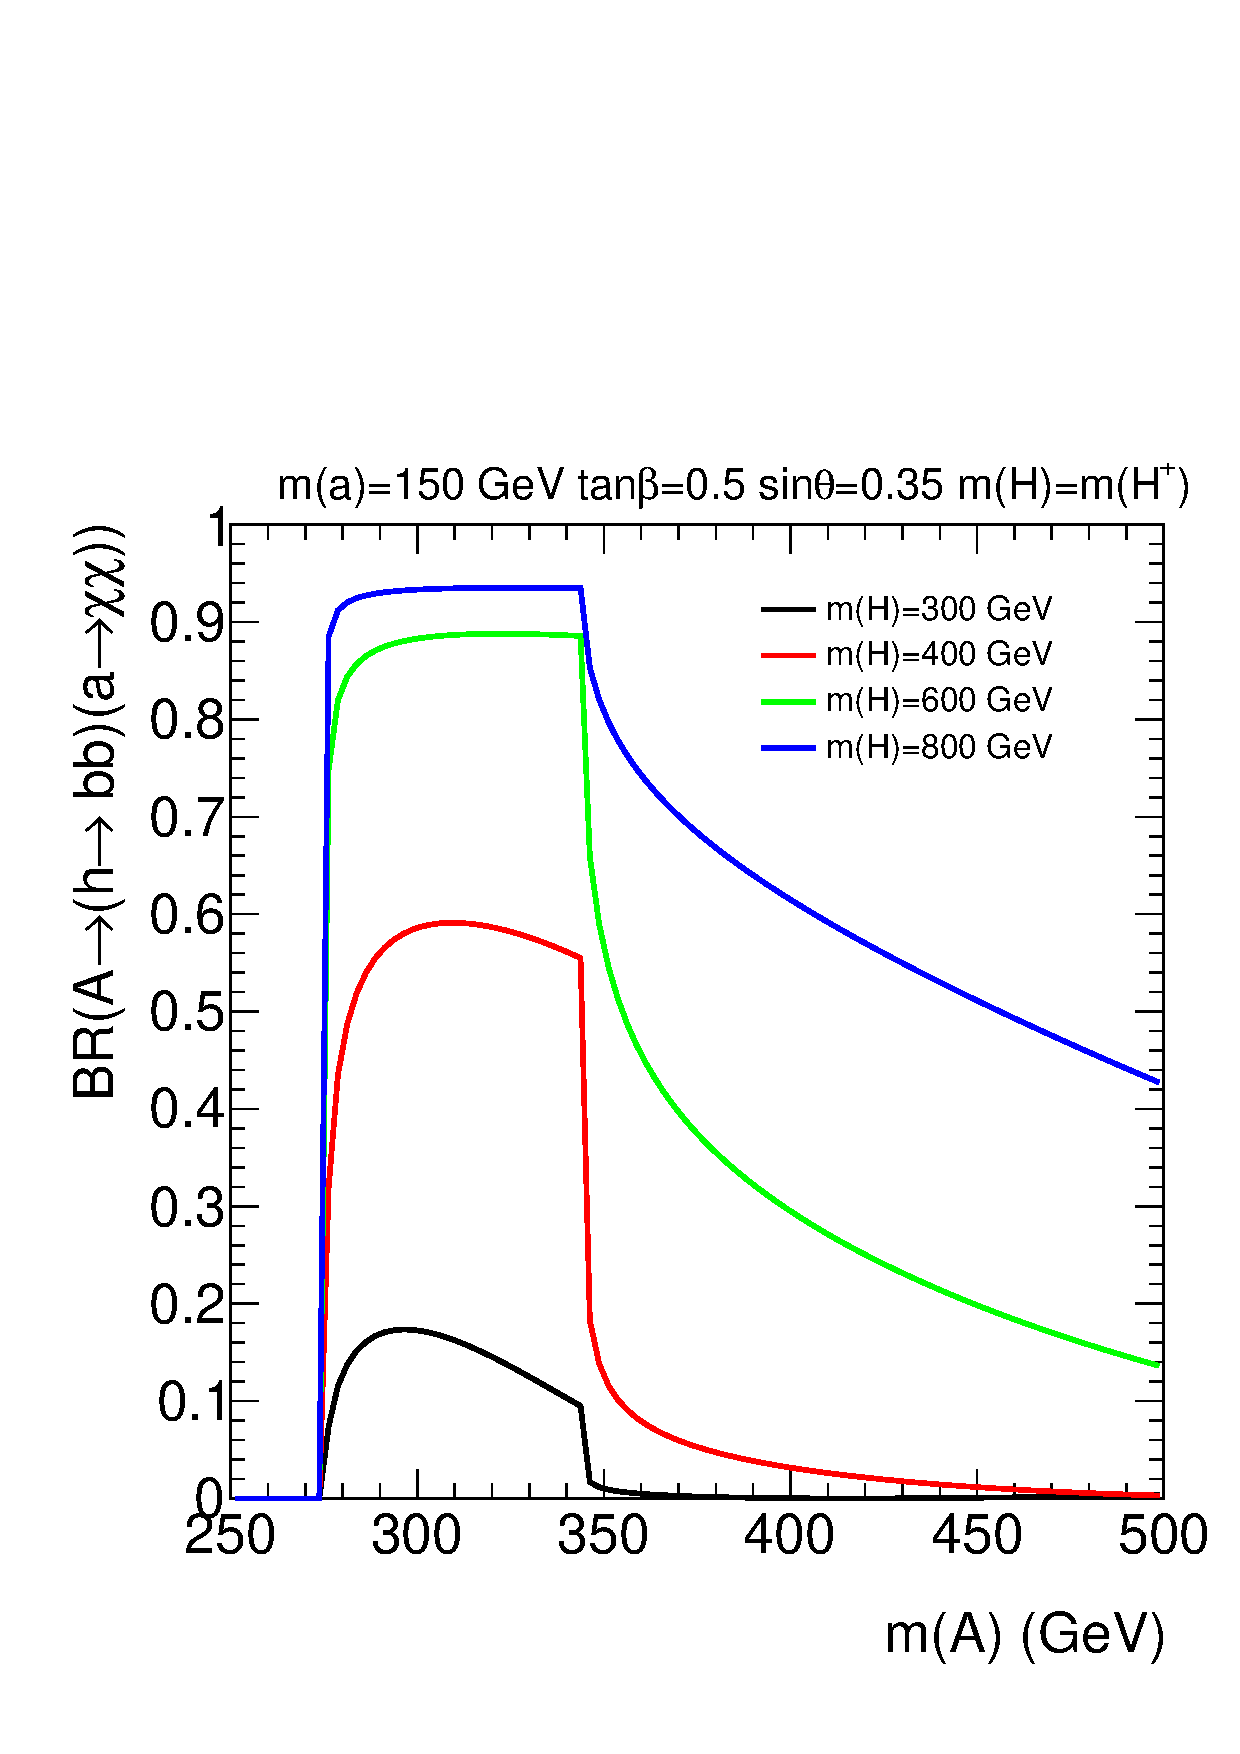
\includegraphics[width=.48\textwidth]{texinputs/04_grid/figures/DMHF/brA}
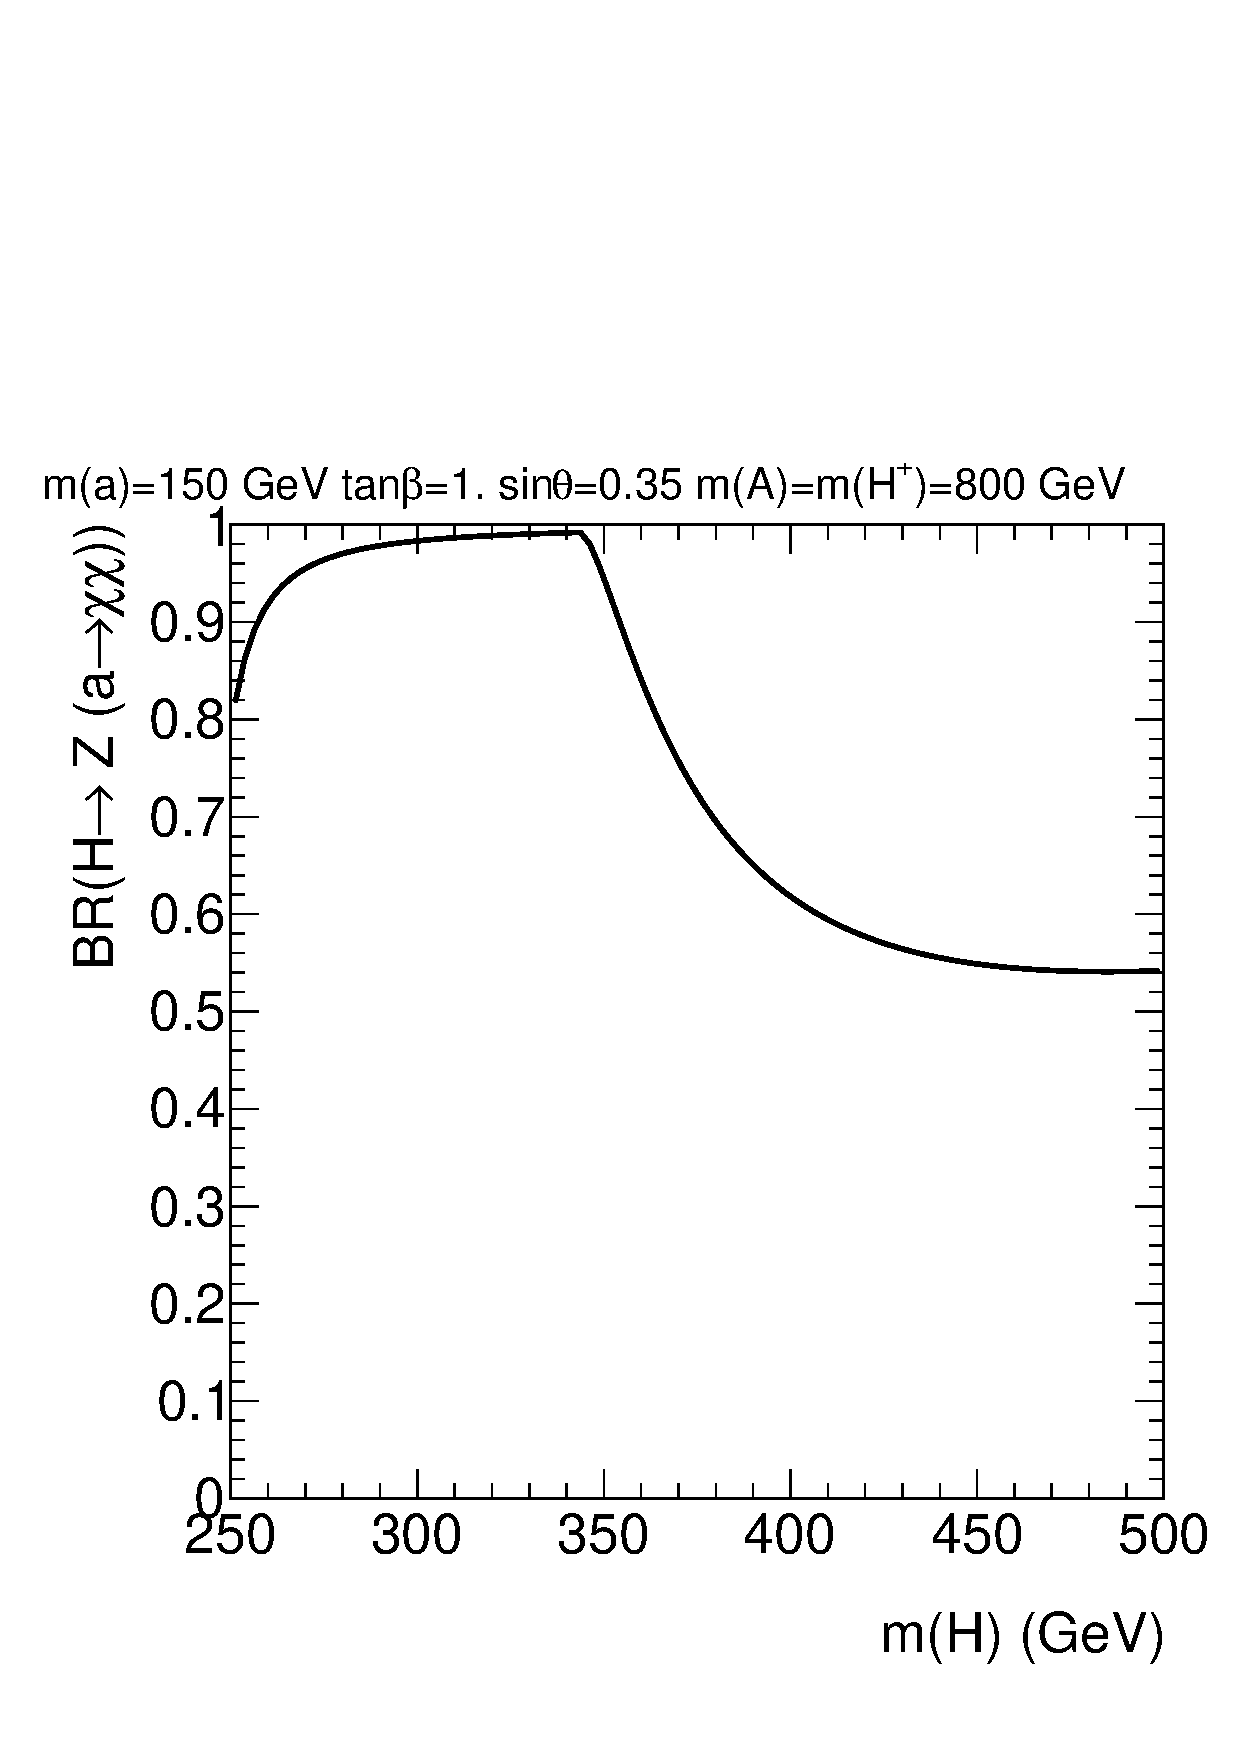
\includegraphics[width=.48\textwidth]{texinputs/04_grid/figures/DMHF/brH}
\caption{Example of the dependence of the $A$ and $H$ branching ratio into $ah$ as a function of some parameters of the 2HDM model.}
\label{fig:brAHah}
\end{figure}

\subsubsection{$tW$+\met signature}

The sensitivity of the LHC experiments to the associated production of dark matter with a single top has been recently studied \cite{Pani:2017qyd} in the framework of an extension of the standard model featuring two Higgs doublets and an additional pseudoscalar mediator. 
This study extends the work of previous literature \cite{Pinna:2017tay}, which demonstrated using a simplified model that considering final states involving a single top quark and DM (DM$t$) increases the coverage of existing analyses targeting DM particles produced in association with $t\bar t$.  

\begin{figure}
\begin{center}
\begin{subfigure}{.23\textwidth}\centering
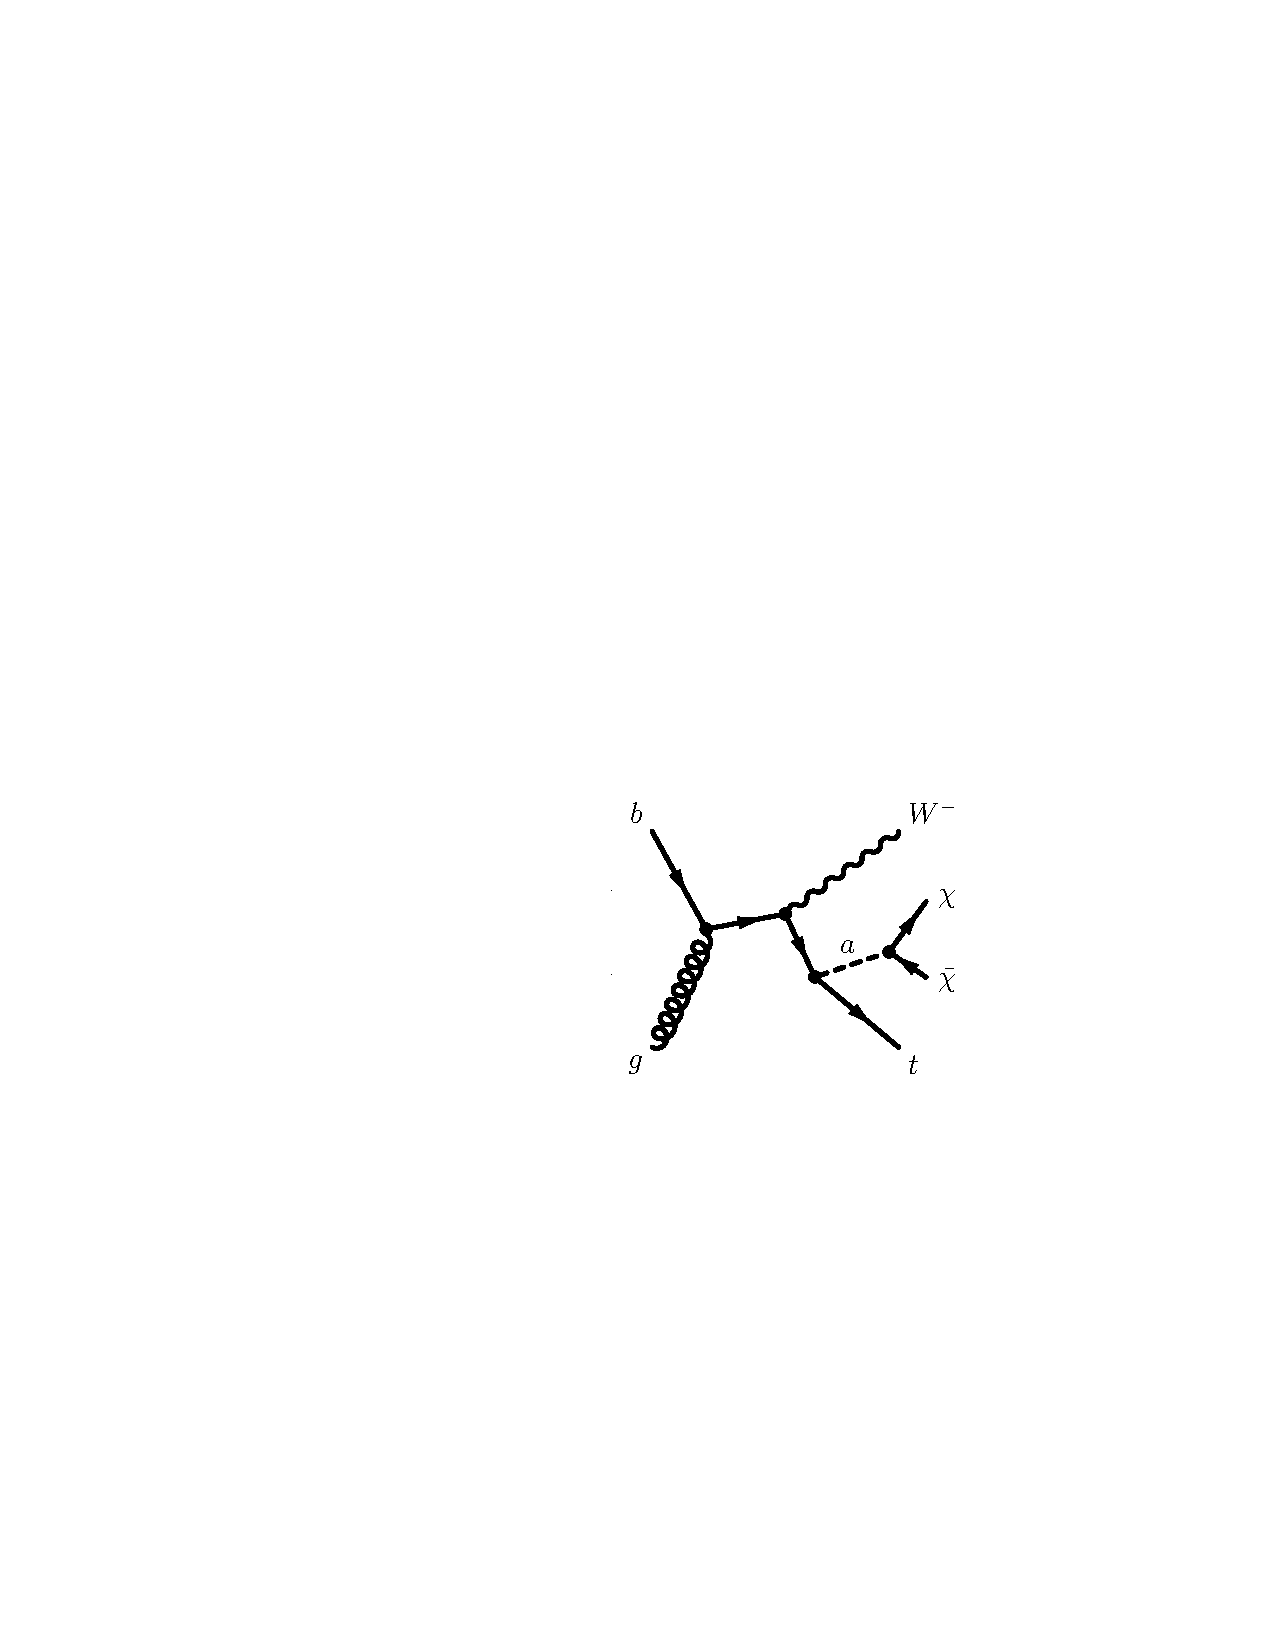
\includegraphics[width=\textwidth]{texinputs/04_grid/figures/DMHF/Pfeyn_tw2}
\caption{}
\end{subfigure}
\begin{subfigure}{.23\textwidth}\centering
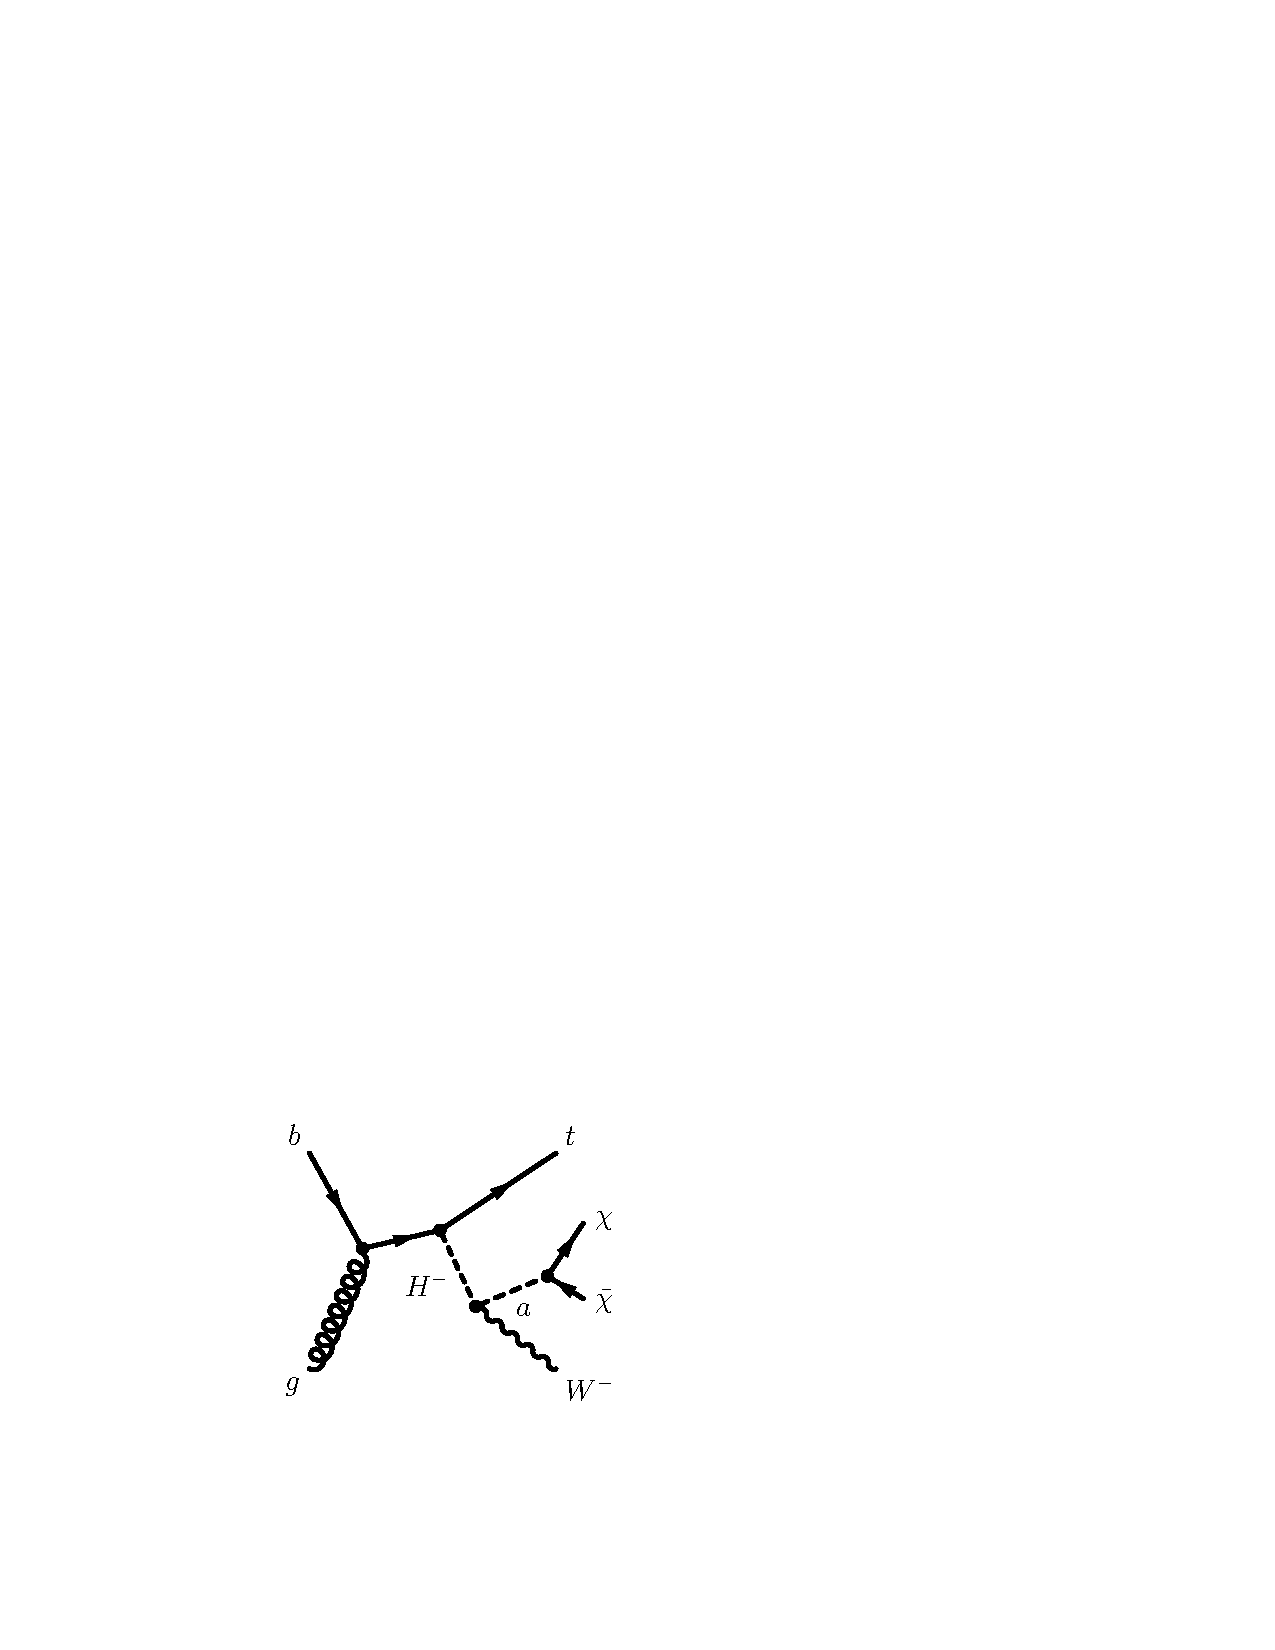
\includegraphics[width=\textwidth]{texinputs/04_grid/figures/DMHF/Pfeyn_tw1}
\caption{}
\end{subfigure}
\begin{subfigure}{.23\textwidth}\centering
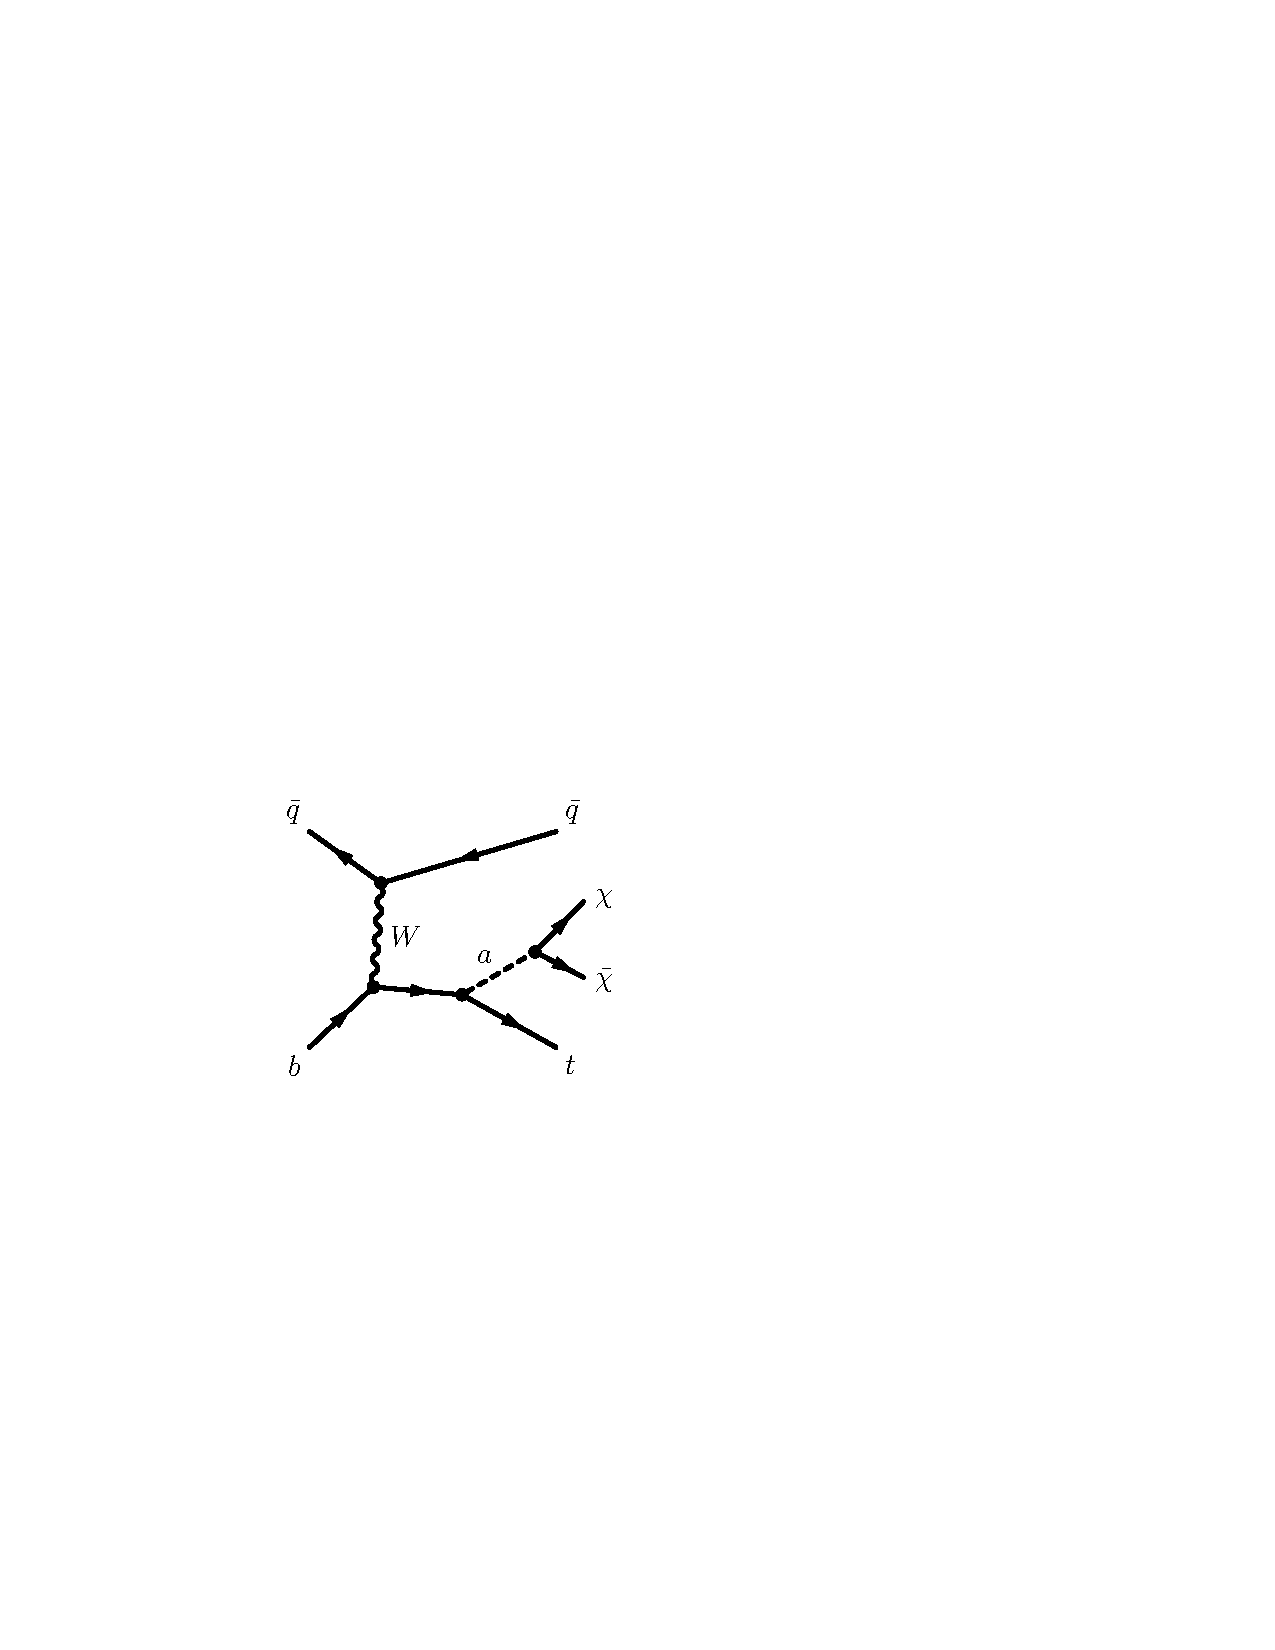
\includegraphics[width=\textwidth]{texinputs/04_grid/figures/DMHF/Pfeyn_tchan_1}
\caption{}
\end{subfigure}
\begin{subfigure}{.23\textwidth}\centering
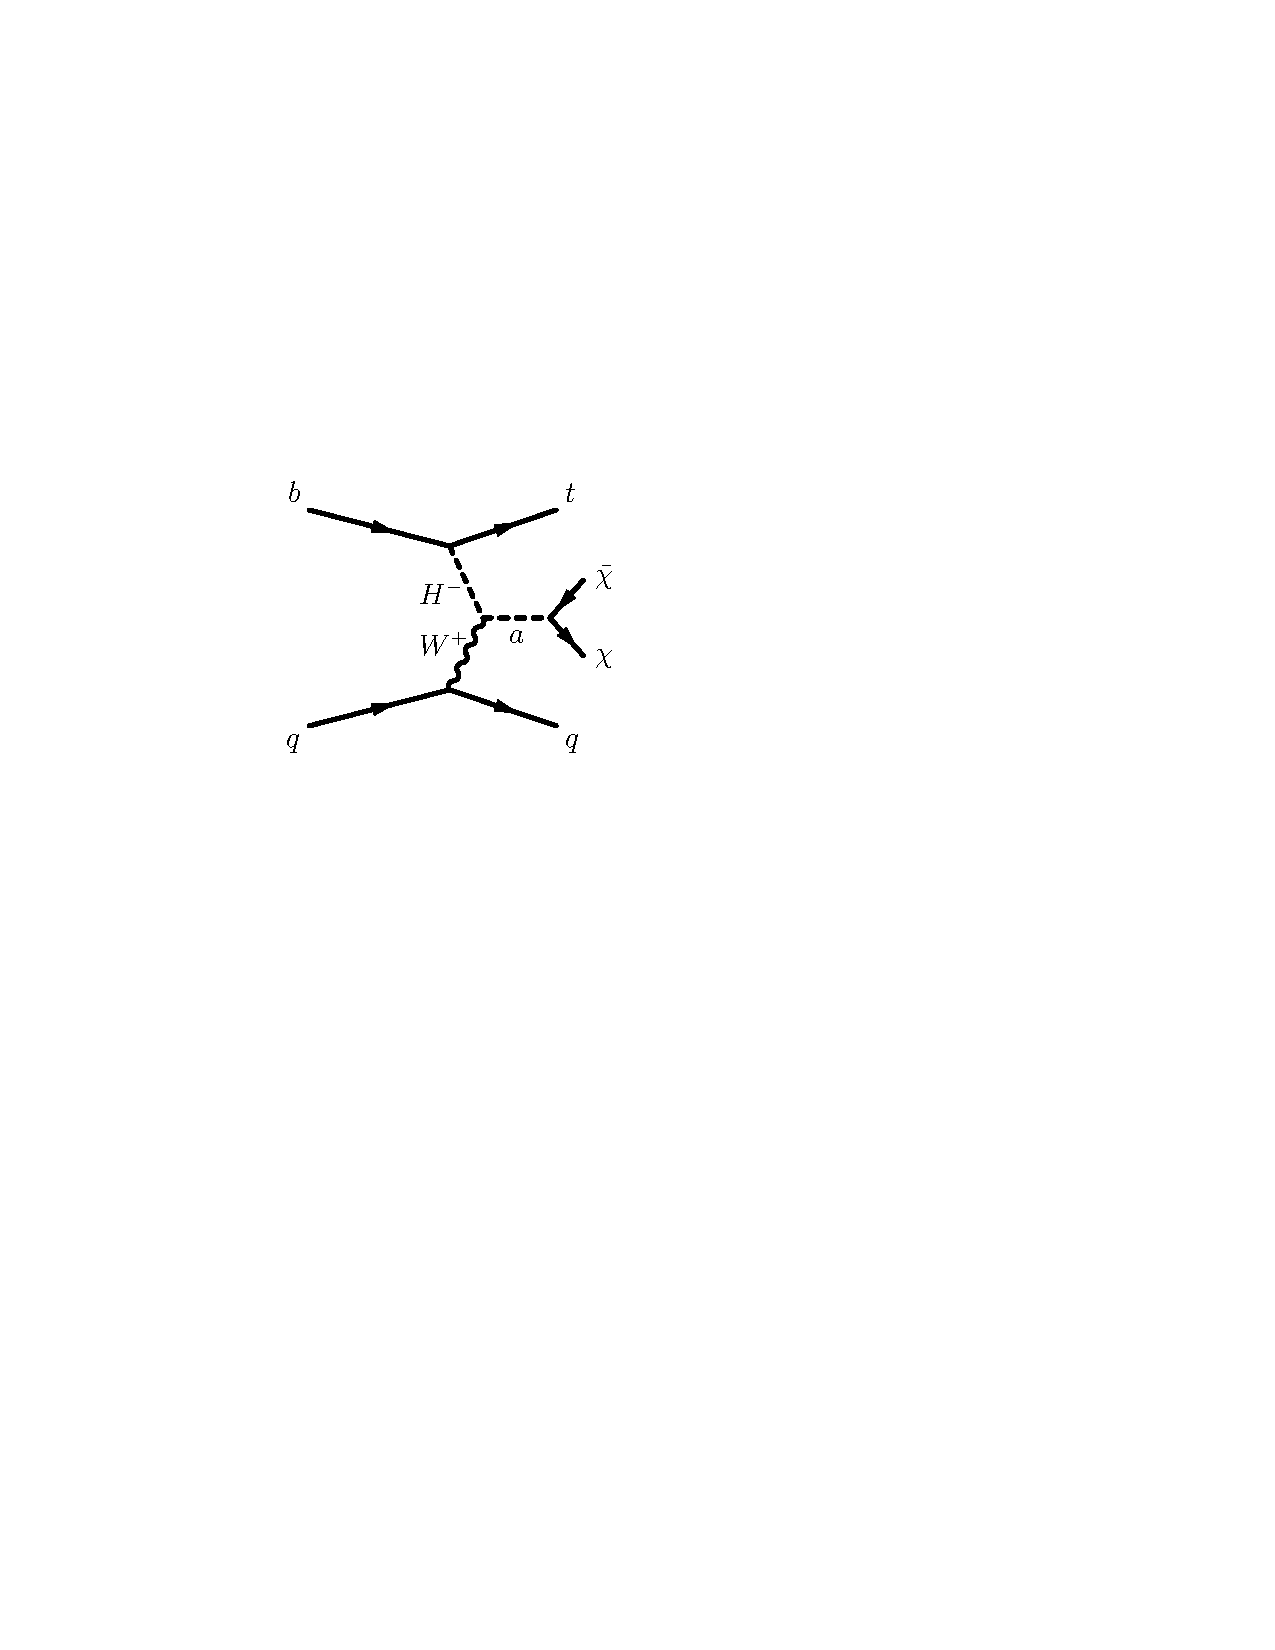
\includegraphics[width=\textwidth]{texinputs/04_grid/figures/DMHF/Pfeyn_tchan_2}
\caption{}
\end{subfigure}
\caption{Representative diagrams for $tW$ and $t$-channel production of DM in association with a single top quark.}
%($pp \rightarrow tj\chi\chi$)}
\label{fig:feyn1}
\end{center}
\end{figure}

Like single top production within the SM, the DM$t$ signature in the model includes three different types of contributions at leading order (LO) in QCD: $t$-channel production, $s$-channel production and associated production together with a $W$ boson ($tW$) (Fig.~\ref{fig:feyn1}).
When the decay $H^{\pm}\rightarrow W^{\pm} a$ is possible, the $H^{\pm}$ is produced on-shell, and the cross-section of $pp \rightarrow tW\chi\chi$, 
assuming $H^{\pm}$ masses of a few hundred \GeV, is around one order of magnitude larger than the one for the same process in the simplified model. Moreover the production and cascade decay of a resonance yields kinematic signatures which can be exploited to separate the signal from the SM background. 

Ref.~\cite{Pani:2017qyd} analyzes detector-smeared generator-level signal and background samples using dedicated selections considering one and two lepton final states, in order to assess the coverage in parameter space for this signature at a centre-of-mass energy of 14 TeV assuming an integrated luminosity of 300~fb$^{-1}$. 
%Background and signal Monte Carlo simulated samples are employed for the estimate of the results. The effect of the detector on the kinematic quantities utilised in the analysis is simulated by applying a Gaussian smearing to the momenta of the different reconstructed objects and reconstruction and tagging efficiency factors.
\autoref{DMHF:monotopres} shows the reach of this signature for two of the parameter scans proposed in this whitepaper, in the ($\ma,\tan\beta$) plane assuming $\sin\theta$ = 0.35 and $m(A) = m(H^\pm) = m(H) = 500$ GeV, and as a function of $\tan\beta$ assuming $sin\theta = 0.35$, $m(a)$ = 150 GeV and $m(A) = m(H^\pm) = m(H) = 500$ GeV. 
The sensitivity of this signature is comparable to the one of the Higgs + \MET signature~\cite{Bauer:2017ota}. 
%The results are derived from the simulated samples using a
%re-scaling  procedure described in Ref.[IN PREPARATION]
%In this signature, the sensitivity reach is comparable to the one from the mono-h signature as presented in Ref.~\cite{Bauer:2017ota}. 

\begin{figure}
\centering
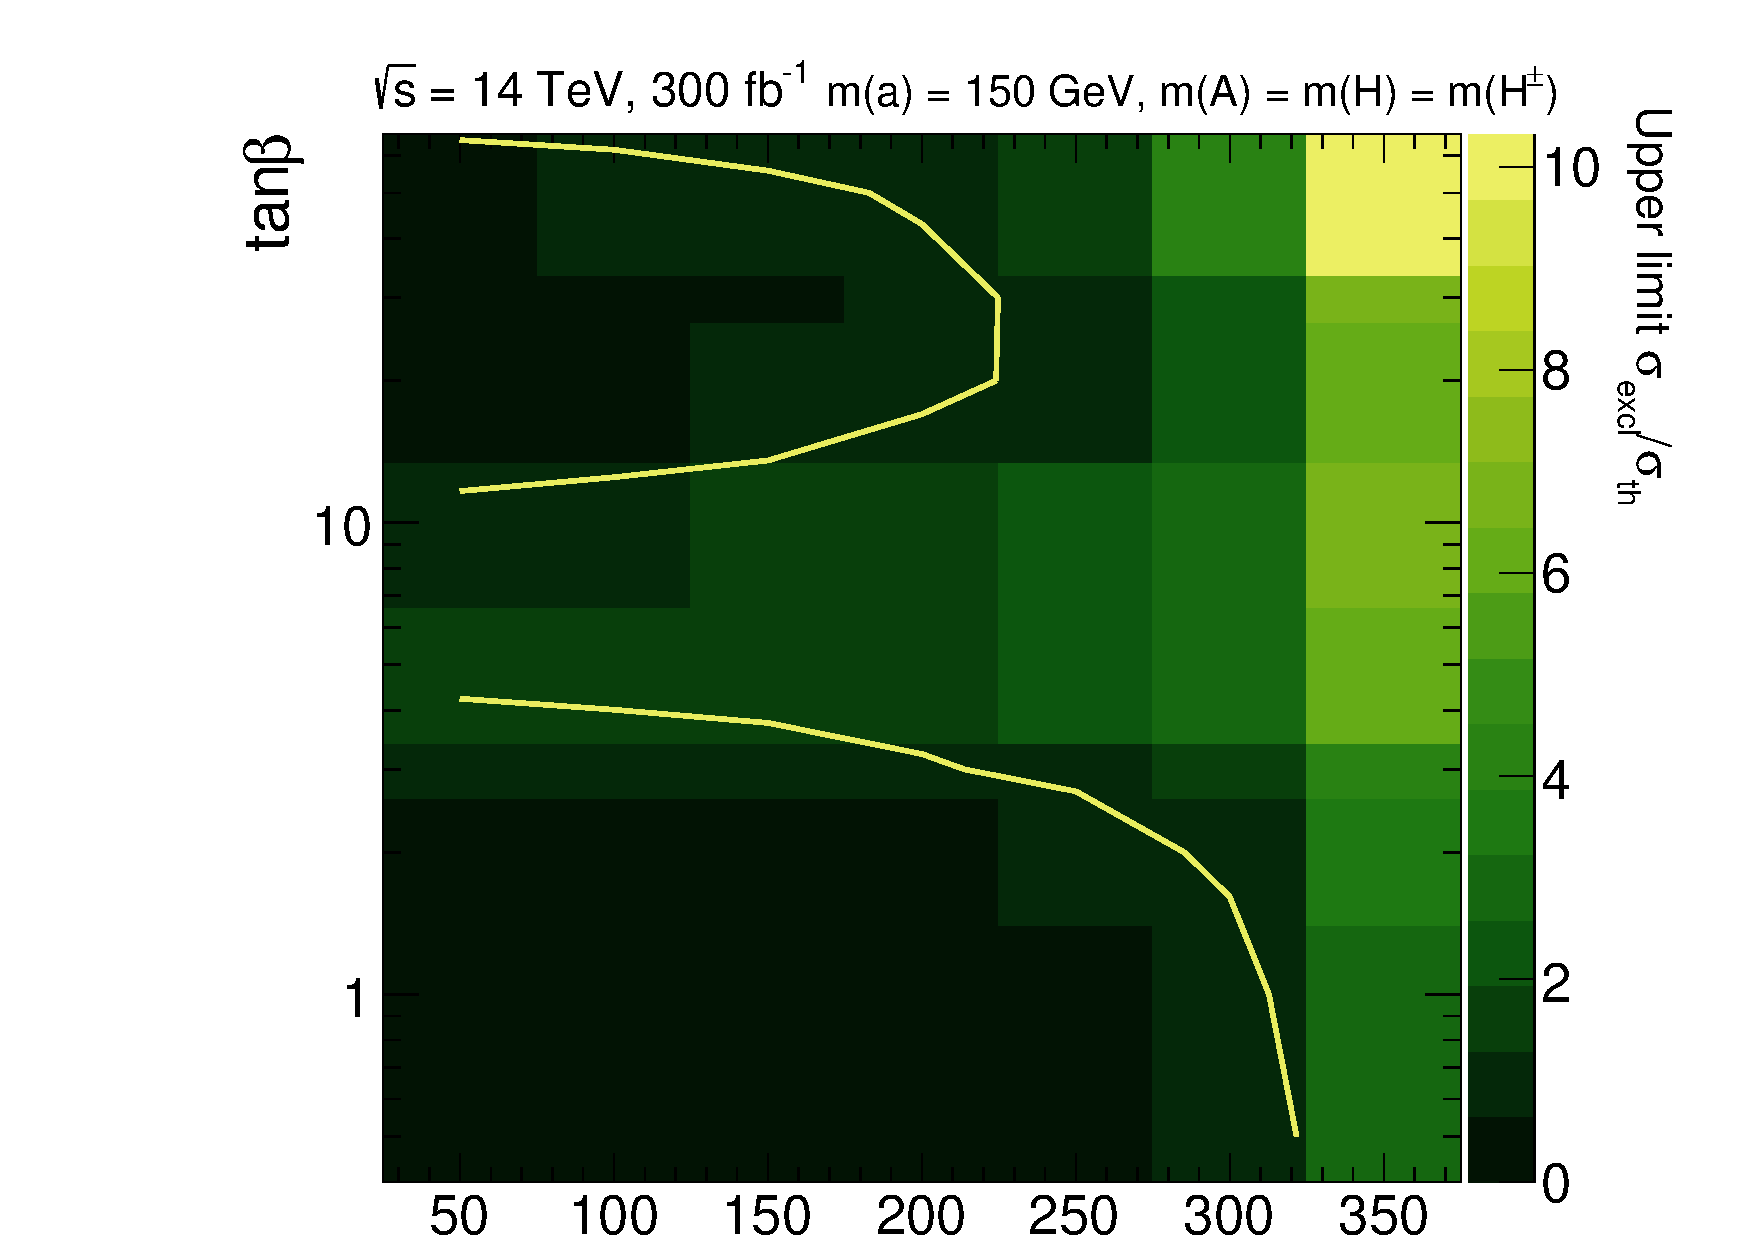
\includegraphics[width=.48\textwidth]{texinputs/04_grid/figures/DMHF/SRrec2l_2DSCAN_a}
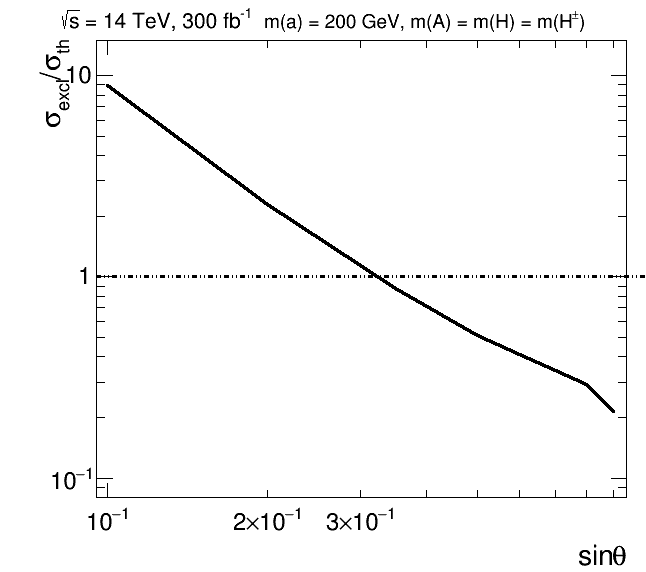
\includegraphics[width=.47\textwidth]{texinputs/04_grid/figures/DMHF/SR2la_ULscan4}
\caption{Sensitivity in terms of excluded/theoretical cross-section for the tW+\met signature in the ($m(a)$,$\tan\beta$) plane, fixing $m(a)$ to 150 GeV, $sin\theta = 0.35$ and $m(A) = m(H^\pm) = m(H)$ (left). Sensitivity as a function of $\tan\beta$, assuming $sin\theta = 0.35$, $m(a)$ = 150 GeV and $m(A) = m(H^\pm) = m(H) = 500$ GeV (right).}
\label{DMHF:monotopres}
\end{figure}


\subsubsection{\ttbar\ resonances}

Heavy (pseudo)scalar bosons with $M_{A/H}\ge2\mt$ and $\tanb \sim \mathcal{O}(1)$ will decay dominantly into top-quark pairs. Searches for features in the \ttbar\ invariant mass spectra are sensitive to this process. 
In this case, interference effects between the signal processes and the SM \ttbar\ production distort the signal shape from a single peak to a peak-dip structure \cite{Carena:2016npr}. 

The results of the first LHC search accounting for this feature in Ref.~\cite{Aaboud:2017hnm} can be reinterpreted in the context of the \hdma, after modifying the \mg model to feature this effect. Since interference between loop-induced and tree-level processes cannot currently be simulated, "Higgs\_Effective\_Couplings\_FormFactor" approach from Ref.~\cite{Aaboud:2017hnm} is adopted, replacing the loop production by an effective vertex. 
Using this approach, it can be verified that the \hdma reduces to a minimal 2HDM when the pseudoscalar mediator $a$ does not mix with the heavy pseudoscalar $A$ ($\sinp=0$): \autoref{fig:ttres_2HDMvs2HDMa} shows the \ttbar\ invariant mass distribution in both cases, showing the peak-dip structure. 

While a full study of the sensitivity of this search is not shown in this whitepaper, examples of how its reach changes as a function of the parameters of the \hdma, the $M_{\ttbar}$ signal distribution are presented in Fig~\ref{fig:ttres_2HDM_A}. Larger values of \tanb\ or \sinp\ are expected to yield lower sensitivities to $A\rightarrow\ttbar$ significantly while \ma\ almost only affects the contribution from $a\rightarrow\ttbar$, which becomes sizeable if \ma is close to $2\mt$.

\begin{figure}
\centering
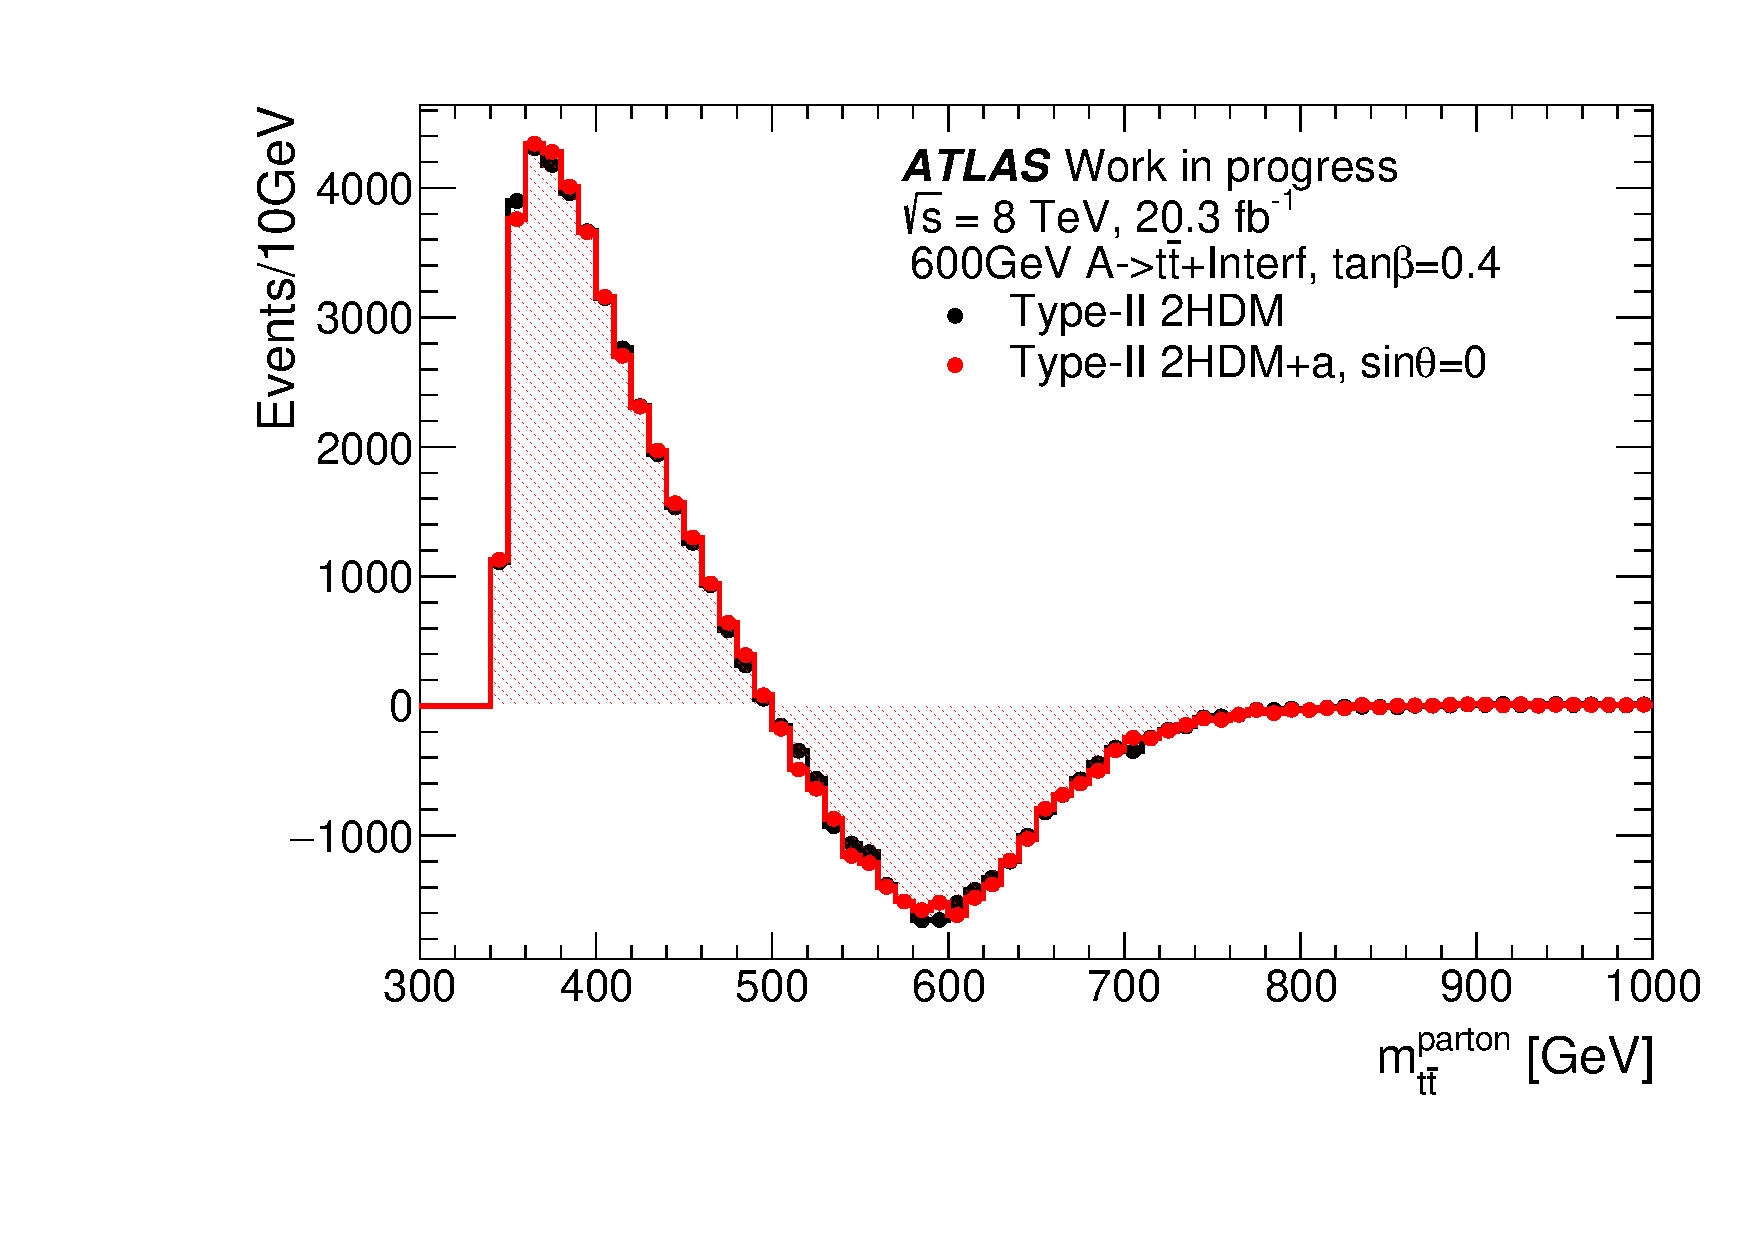
\includegraphics[width=.48\textwidth]{texinputs/04_grid/figures/ttres/ttres_2HDMvs2HDMa_A.pdf}
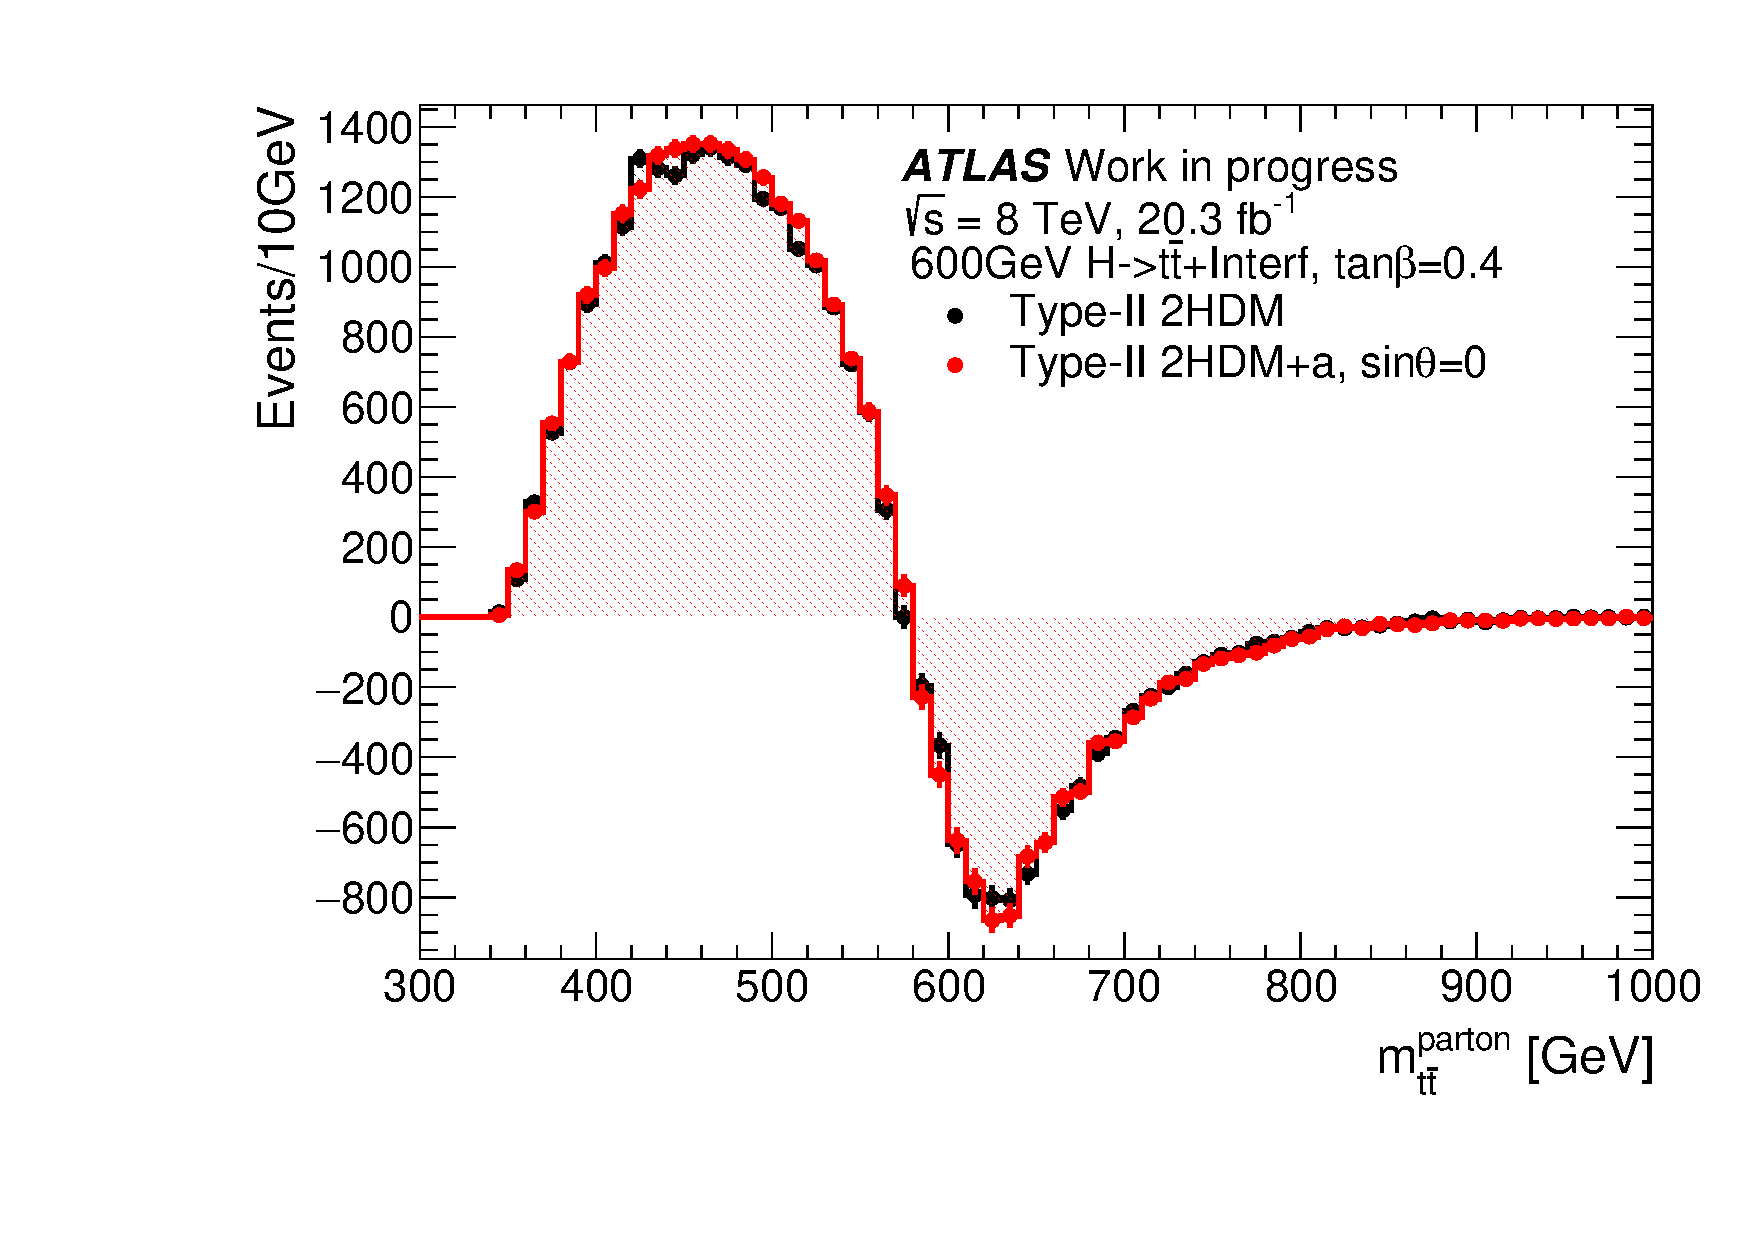
\includegraphics[width=.48\textwidth]{texinputs/04_grid/figures/ttres/ttres_2HDMvs2HDMa_H.pdf}
\caption{$M_{\ttbar}$ distribution of the heavy (pseudo)scalar boson decaying into \ttbar\ with $\mA=\mH=600\GeV, \tanb=0.4$, $\sinp=1/\sqrt{2}$ and $M_a=100\GeV$ in comparison with the one from the generic 2HDM.}
\label{fig:ttres_2HDMvs2HDMa}
\end{figure}

\begin{figure}
\centering
\begin{subfigure}[b]{0.49\textwidth}
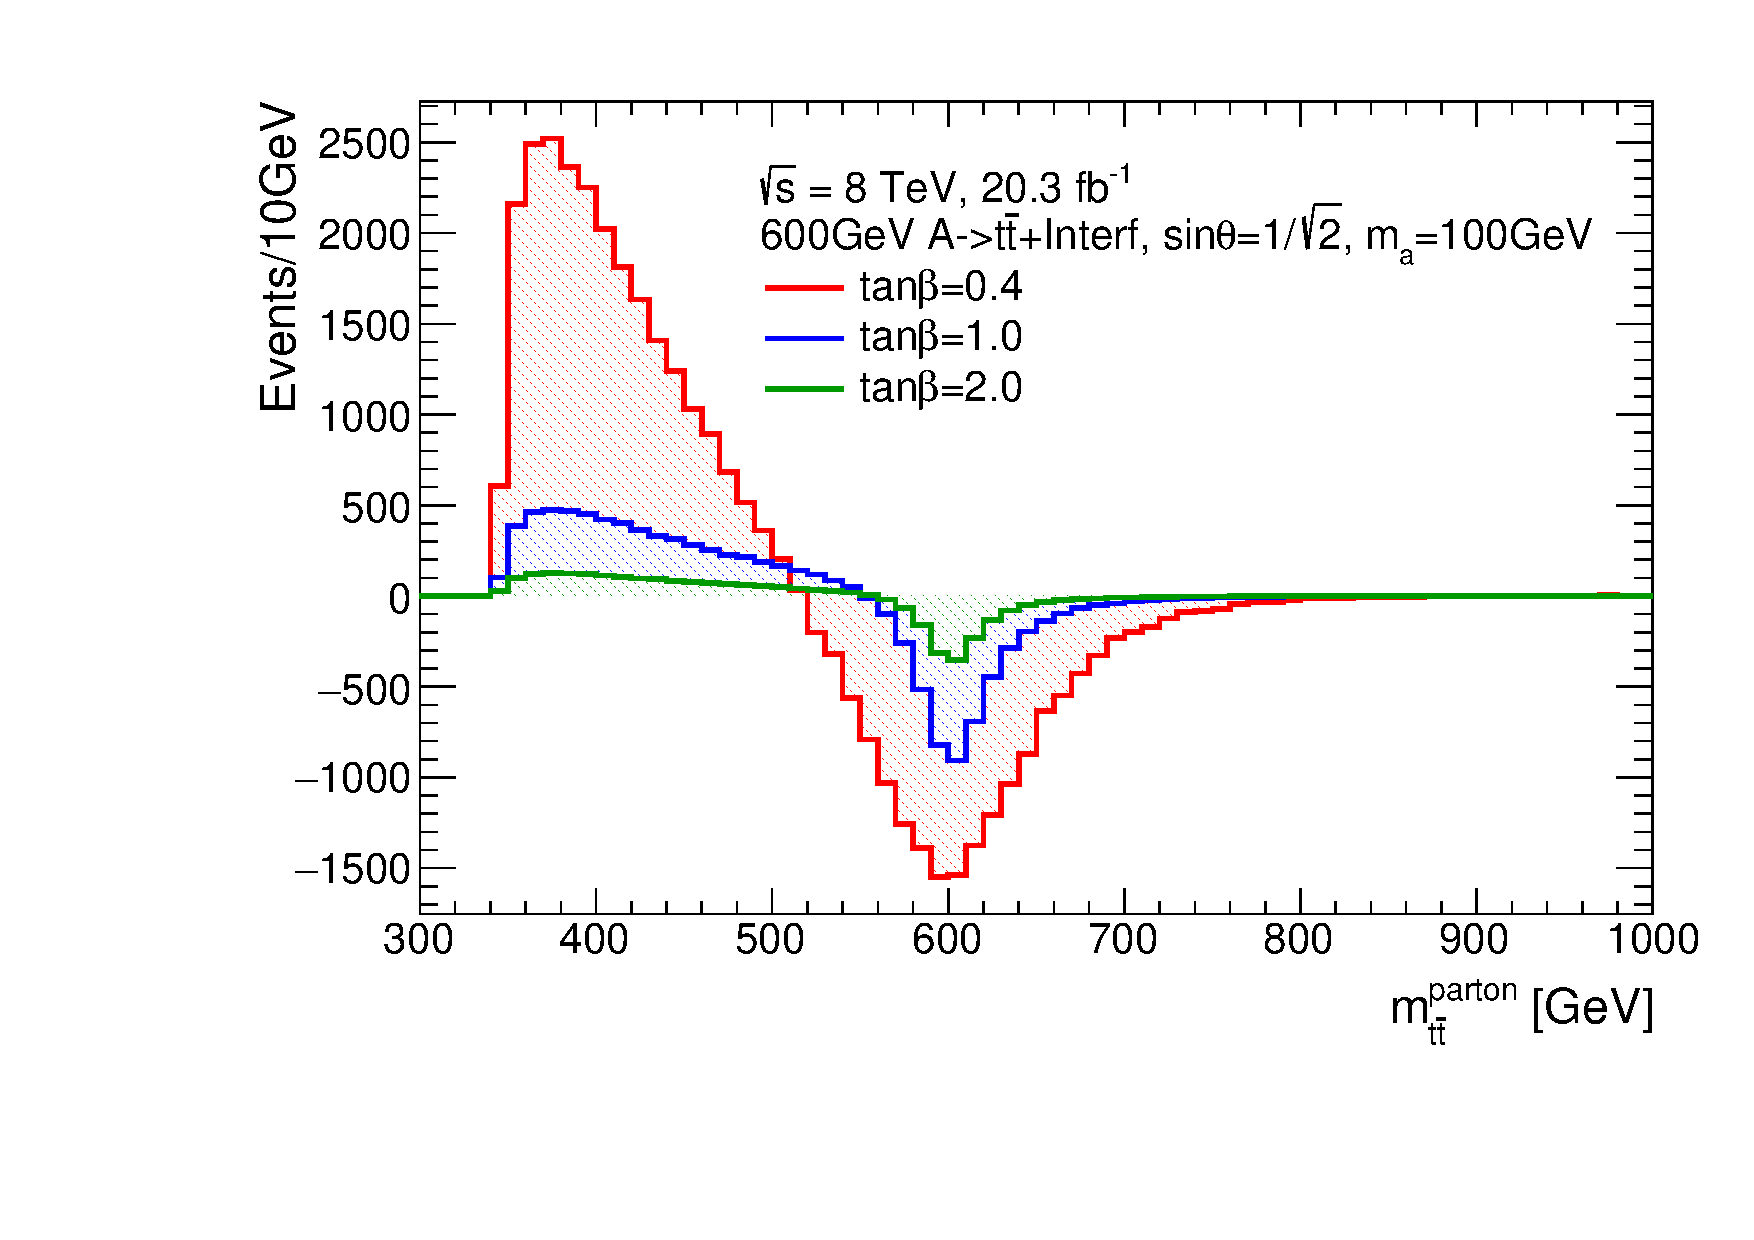
\includegraphics[width=\textwidth]{texinputs/04_grid/figures/ttres/ttres_2HDMa_A_tanb.pdf}
\caption{\tanb dependency with fixed $\sinp=1/\sqrt{2}$ and $\ma=100\GeV$}
\end{subfigure}
\begin{subfigure}[b]{0.49\textwidth}
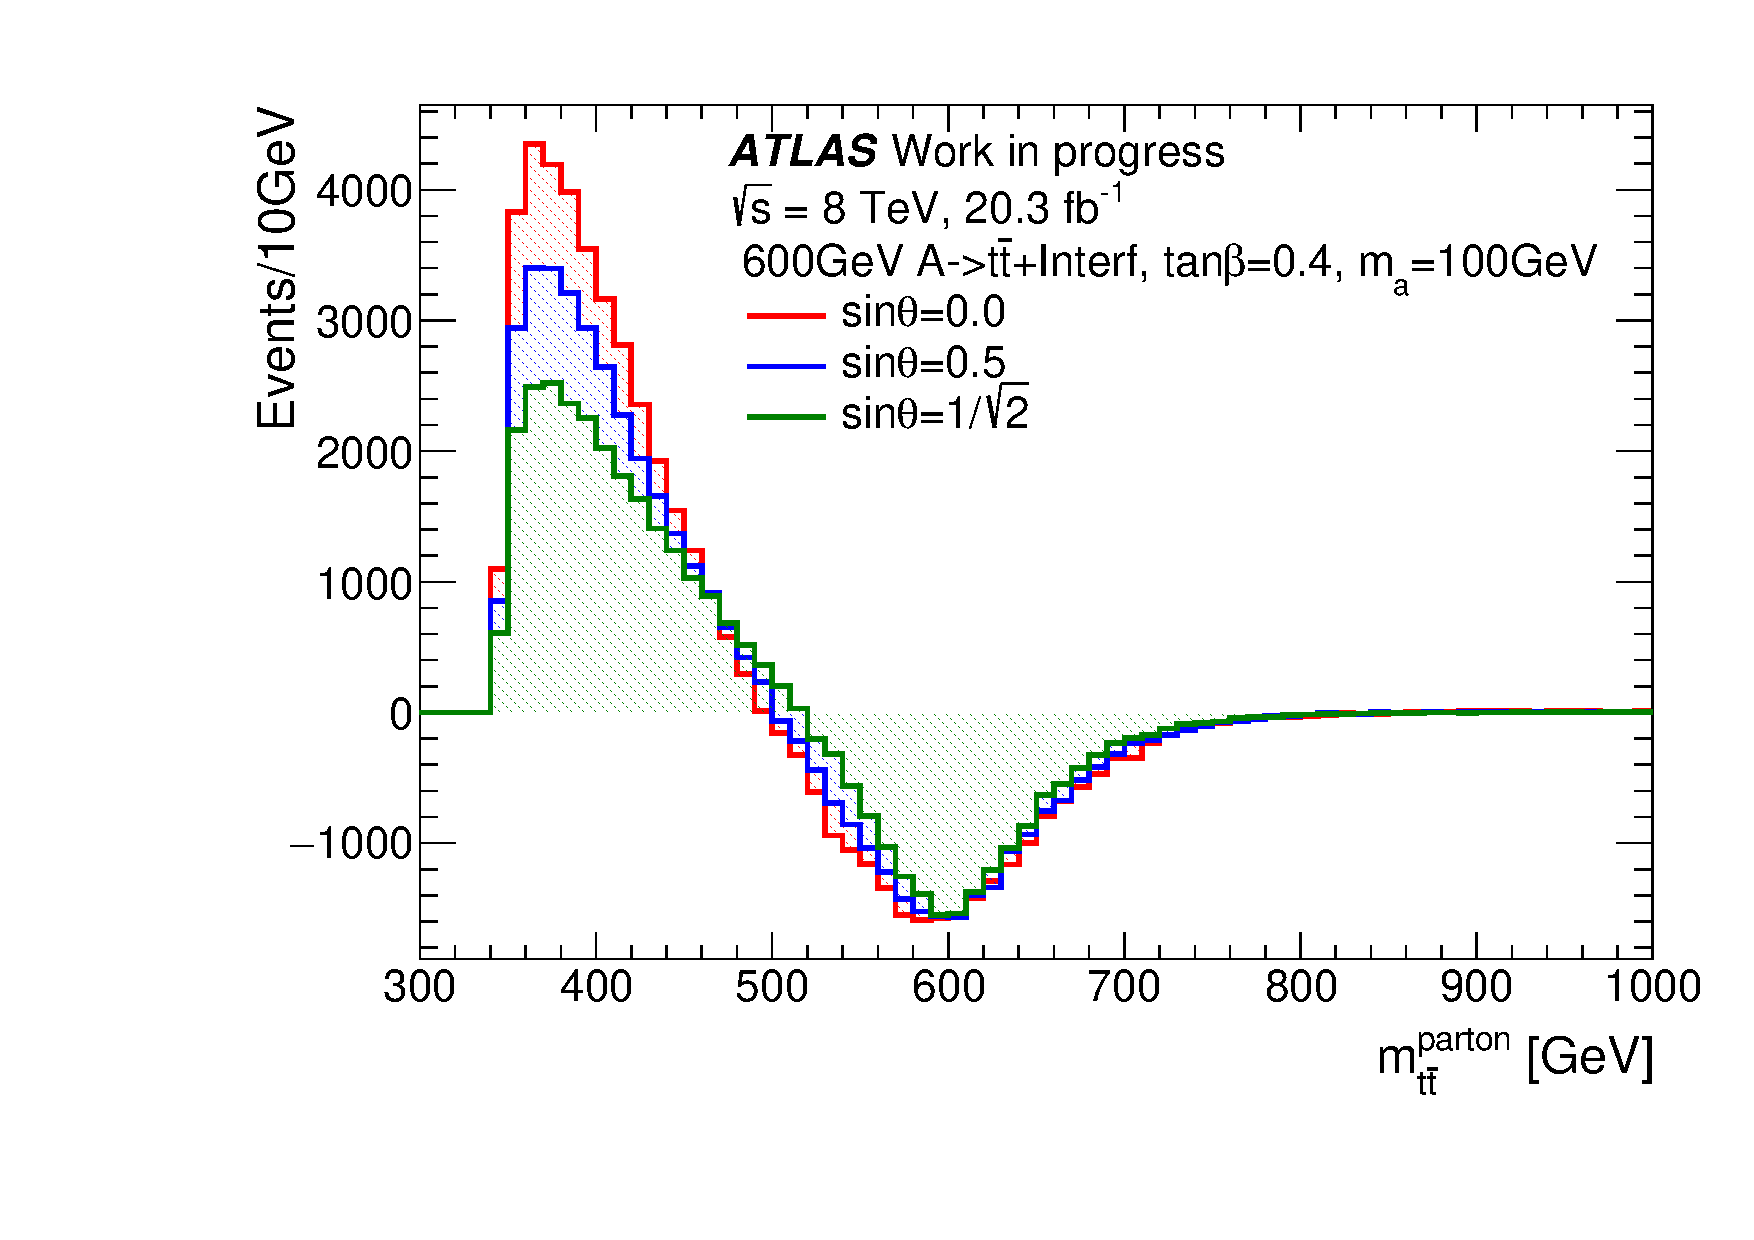
\includegraphics[width=\textwidth]{texinputs/04_grid/figures/ttres/ttres_2HDMa_A_sinp.pdf}
\caption{\sinp dependency with fixed $\tanb=0.4$ and $\ma=100\GeV$}
\end{subfigure}
\begin{subfigure}[b]{0.49\textwidth}
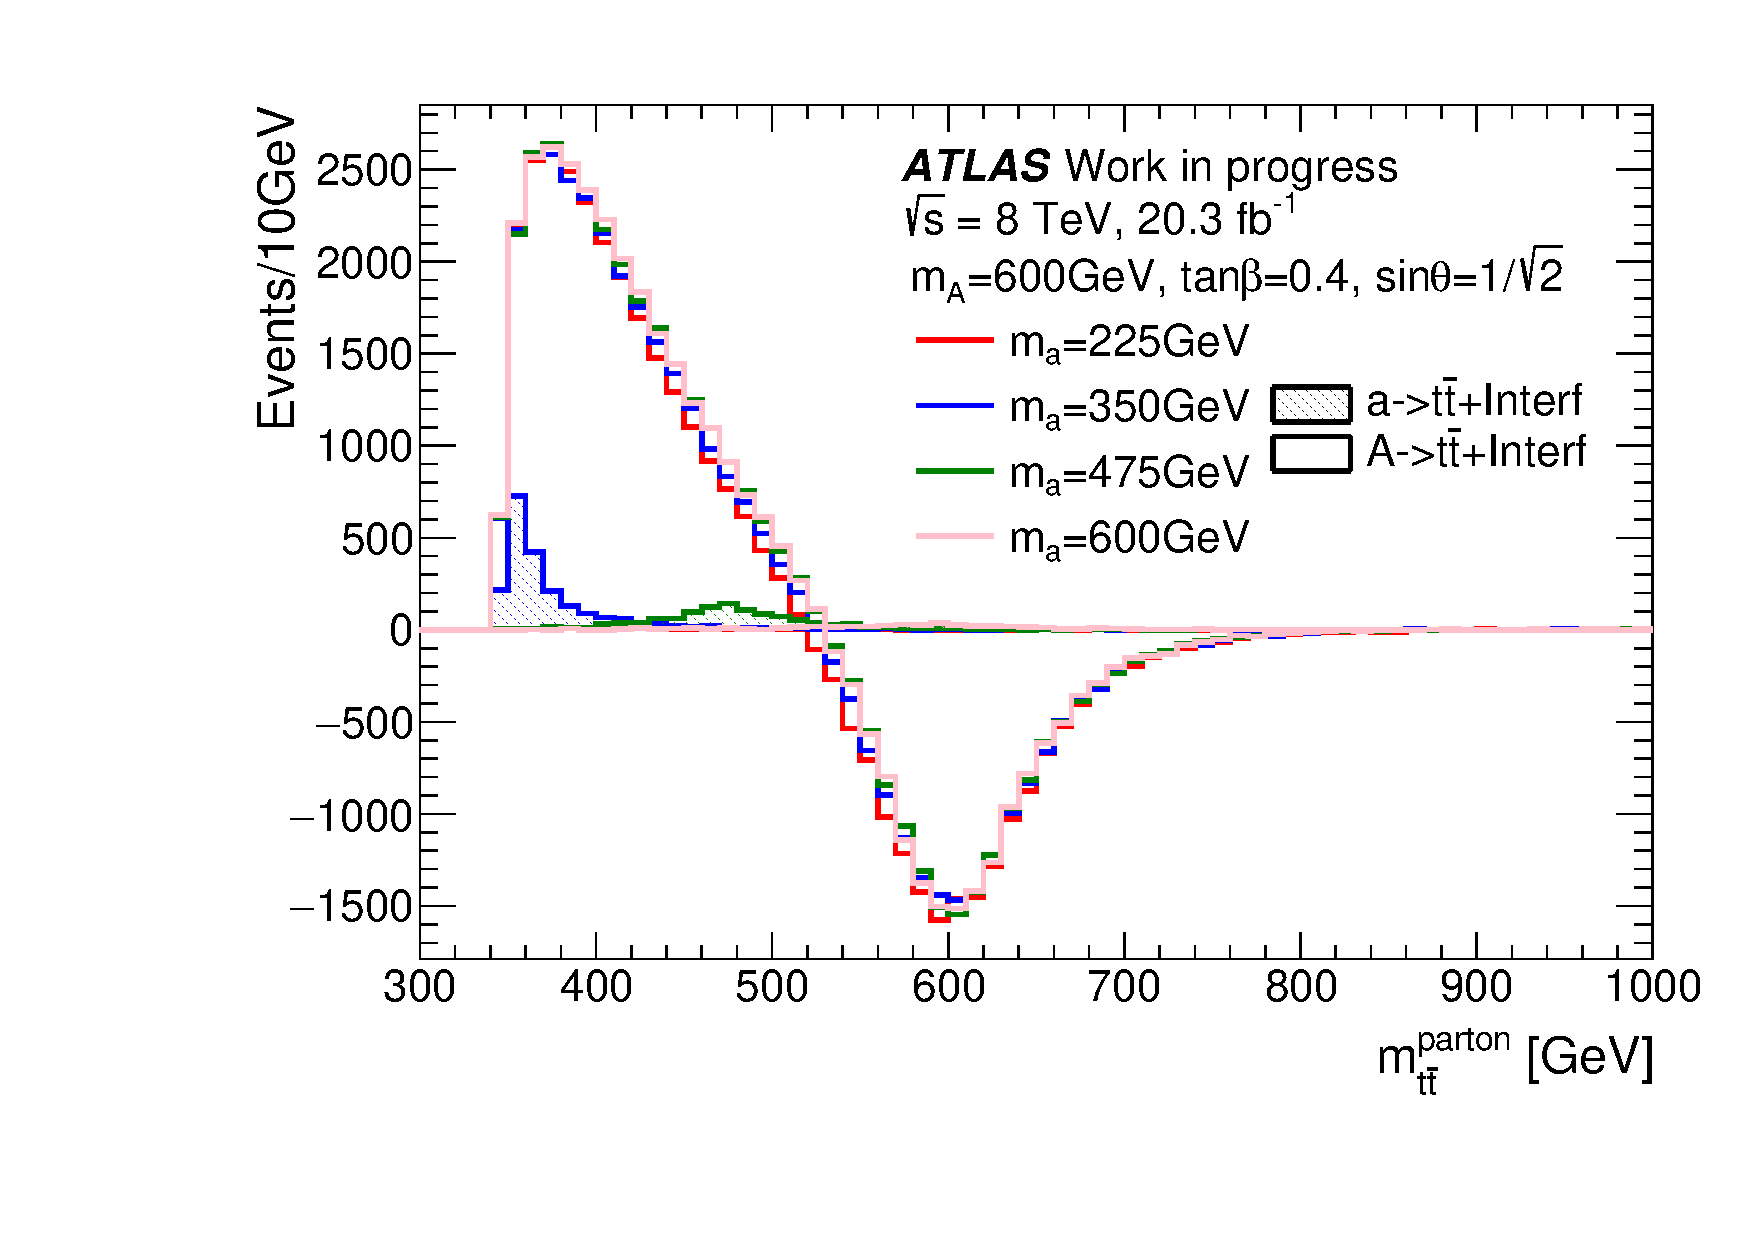
\includegraphics[width=\textwidth]{texinputs/04_grid/figures/ttres/ttres_2HDMa_A_ma.pdf}
\caption{\ma dependency with fixed $\tanb=0.4$ and $\sinp=1/\sqrt{2}$}
\end{subfigure}
\caption{Signal $M_{\ttbar}$ distribution as a function of various model parameters. The value of \mA is fixed at 600\GeV.}
\label{fig:ttres_2HDM_A}
\end{figure}
\FloatBarrier

\subsubsection{Four-top final states}

The topology involving four top-quarks in the final state is a rare, yet increasingly important signature, which will gain sensitivity and attention with the enlargement of the dataset delivered by the LHC.  

In the attempt to perform a first characterization of this final state for this model, we have studied the predicted cross-section for the four top final state of this model for two sets of parameter choices. 

In Figure~\ref{DMHF-4top-scan1} we present the four top cross section for the parameter choices of \sinp = 0.35, \mA = \mH = \mHc = 600 GeV, for an intermediate choice of mass of the light pseudoscalar ($m(a) = 400$ GeV), as a function of $tan\beta$. 

The total four-top production cross section, which accounts for both SM and new physics (NP) contributions and is indicated as $|SM+NP|^2$ in the legend, is compared with the production cross section contributions separately due to SM and NP terms. 
This is achieved technically by setting a requirement on the number of QCD and QED vertices in madgraph, as indicated in Table~\ref{tab-dmhf-4tops}.
%Removed this sentence: where are they indicated? 
The different contributions from on-shell production of each CP-odd and CP-even mediators associated with a top pair and
decaying into a top pair are also shown in the same figure indicated. 
The dominant contribution is driven by the on-shell production of $A$ and $H$ for all choices of $tan\beta$ in this benchmark. 
In the lower panel of Figure~\ref{DMHF-4top-scan1}, the effect of the interference term between the 2HDM+a and the SM is assessed, and is found to have an impact almost always smaller than 5\% on the inclusive cross-section. Note however that the validity of this statement depends on the selection in the experimental analysis. 

%\textbf{Checking whether true for some fiducial cuts, would be important to add statement or clarify that is is not fully conclusive as it is only inclusive.}

In Figure~\ref{DMHF-4top-scan2} we present instead the cross-section study for a different set of parameter choices, for $sin\theta
= \frac{1}{\sqrt{2}}$ and as a function of the light pseudoscalar mass. 
For these parameter choices, the cross-section is independent of $m(a)$. 
As it can be observed from the on-shell contribution breakdown, at the low-end of the mass spectrum the $\ttbar+a$ production dominates, with a peak at $400$ GeV due to the competition between $a\rightarrow \chi\chi$ and $a\rightarrow \ttbar$ and the natural decreasing of the cross section with the increase of $m(a)$.  
The contribution of $\ttbar+H$ and $\ttbar+A$ processes compensates the latter effect in the higher end of the mass-spectrum, with the turn on starting around $800$ GeV due to the competition between $A/H\rightarrow\ttbar$ and cascade decays of the heavy higgses into the light pseudoscalar mediator ($A\rightarrow ah/H\rightarrow aZ$). 
The little bump at 1 TeV is due to interference effects between the three higgs mediators, which are all set to the same mass for this parameter choice.  
The inclusive production cross-section of the \hdma model is also compared with the one obtained by the \texttt{DMSimp} pseudoscalar implementation. 
In a similar way as for the previous benchmark points, the impact of the SM interference term on the inclusive cross-section is found to be very small ($<2\%$), except for $m(a)$ values close to the top theshold. 

Finally, in Figure~\ref{DMHF-4top-scan3} we compare for a small $\tan\beta$ value, the cross section of four-top production from NP processes (see Tab.~\ref{tab-dmhf-4tops}) of benchmarks \#3a and \#3b. 

This cross-section increases for benchmark \#3b for increasing $sin\theta$, as the production mechanism is dominated by $\ttbar+a(\ttbar)$. 
A different and more flat trend is instead observed for benchmark \#3a, for which the $sin\theta$ dependence is more complex and driven by the branching ratios of $A$ and $H$ in a top pair, as the $a\rightarrow \ttbar$ threshold is closed in this case. 

%For the appendix
\begin{table}
\begin{tabular}{ccm{50mm}}
\toprule
{\sc Madgraph} rule & Legend symbol & Details \\\midrule
\verb| p p > t t~ t t~ / a z h1 QED<=2|& $|SM+NP|^2$ & Four-top production including both SM and NP contributions and their interference. \\\midrule
\verb| p p > t t~ t t~ / a z h1 QCD<=2|& $|NP|^2$ & Four-top production from NP processes, including interference terms among
$A,H,a$. \\\midrule
\verb| p p > t t~ t t~ / a z h1 QED<=0|& $|SM|^2$ & Four-top SM production.\\
\bottomrule
\end{tabular}
\caption{Description of the specific MADGRAPH settings used to derive the different curves of Figs~\ref{DMHF-4top-scan1}~and~\ref{DMHF-4top-scan2}.}
\label{tab-dmhf-4tops}
\end{table}

\begin{figure}
\centering
\begin{subfigure}[b]{0.8\textwidth}
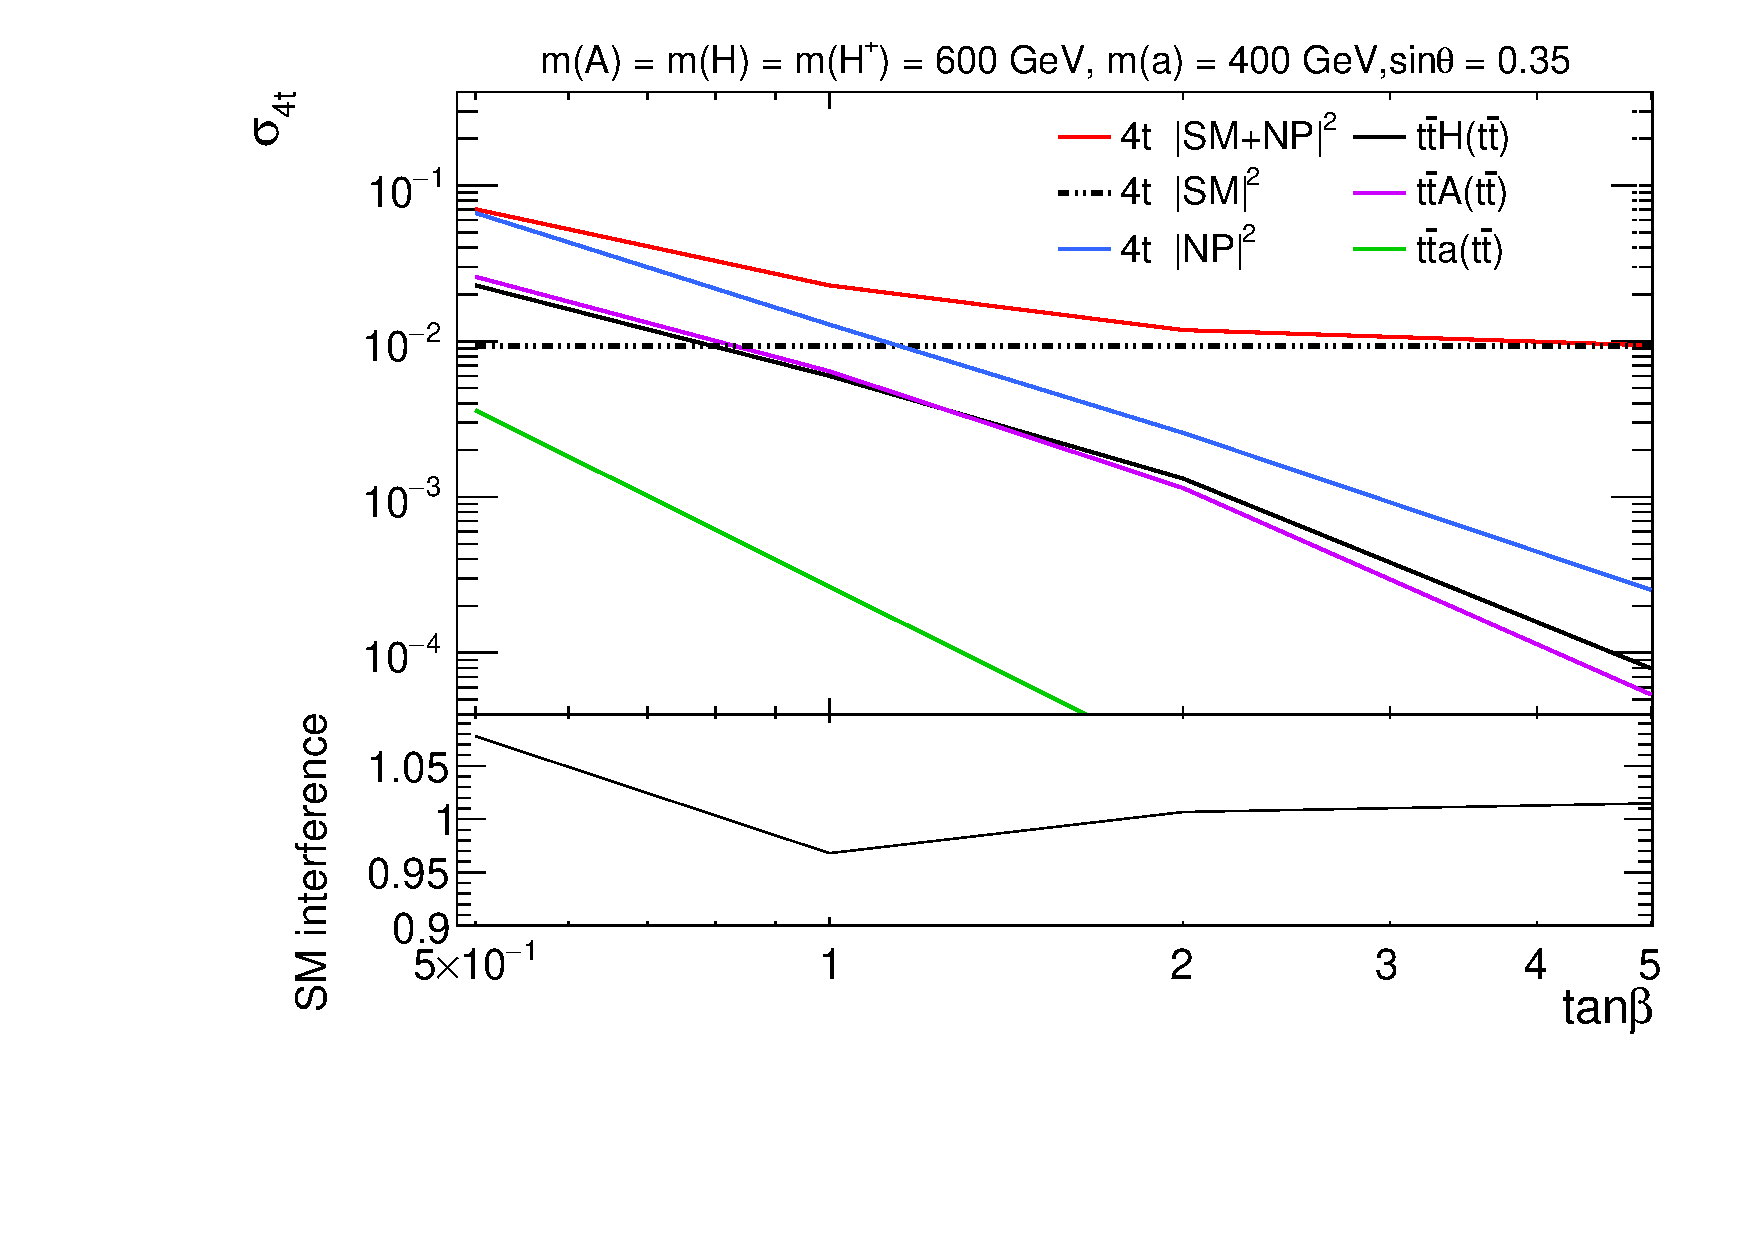
\includegraphics[width=\textwidth]{texinputs/04_grid/figures/DMHF/4tops/WHP_final_tbscan.pdf}
\caption{}
\label{DMHF-4top-scan1}
\end{subfigure}
\begin{subfigure}[b]{0.8\textwidth}
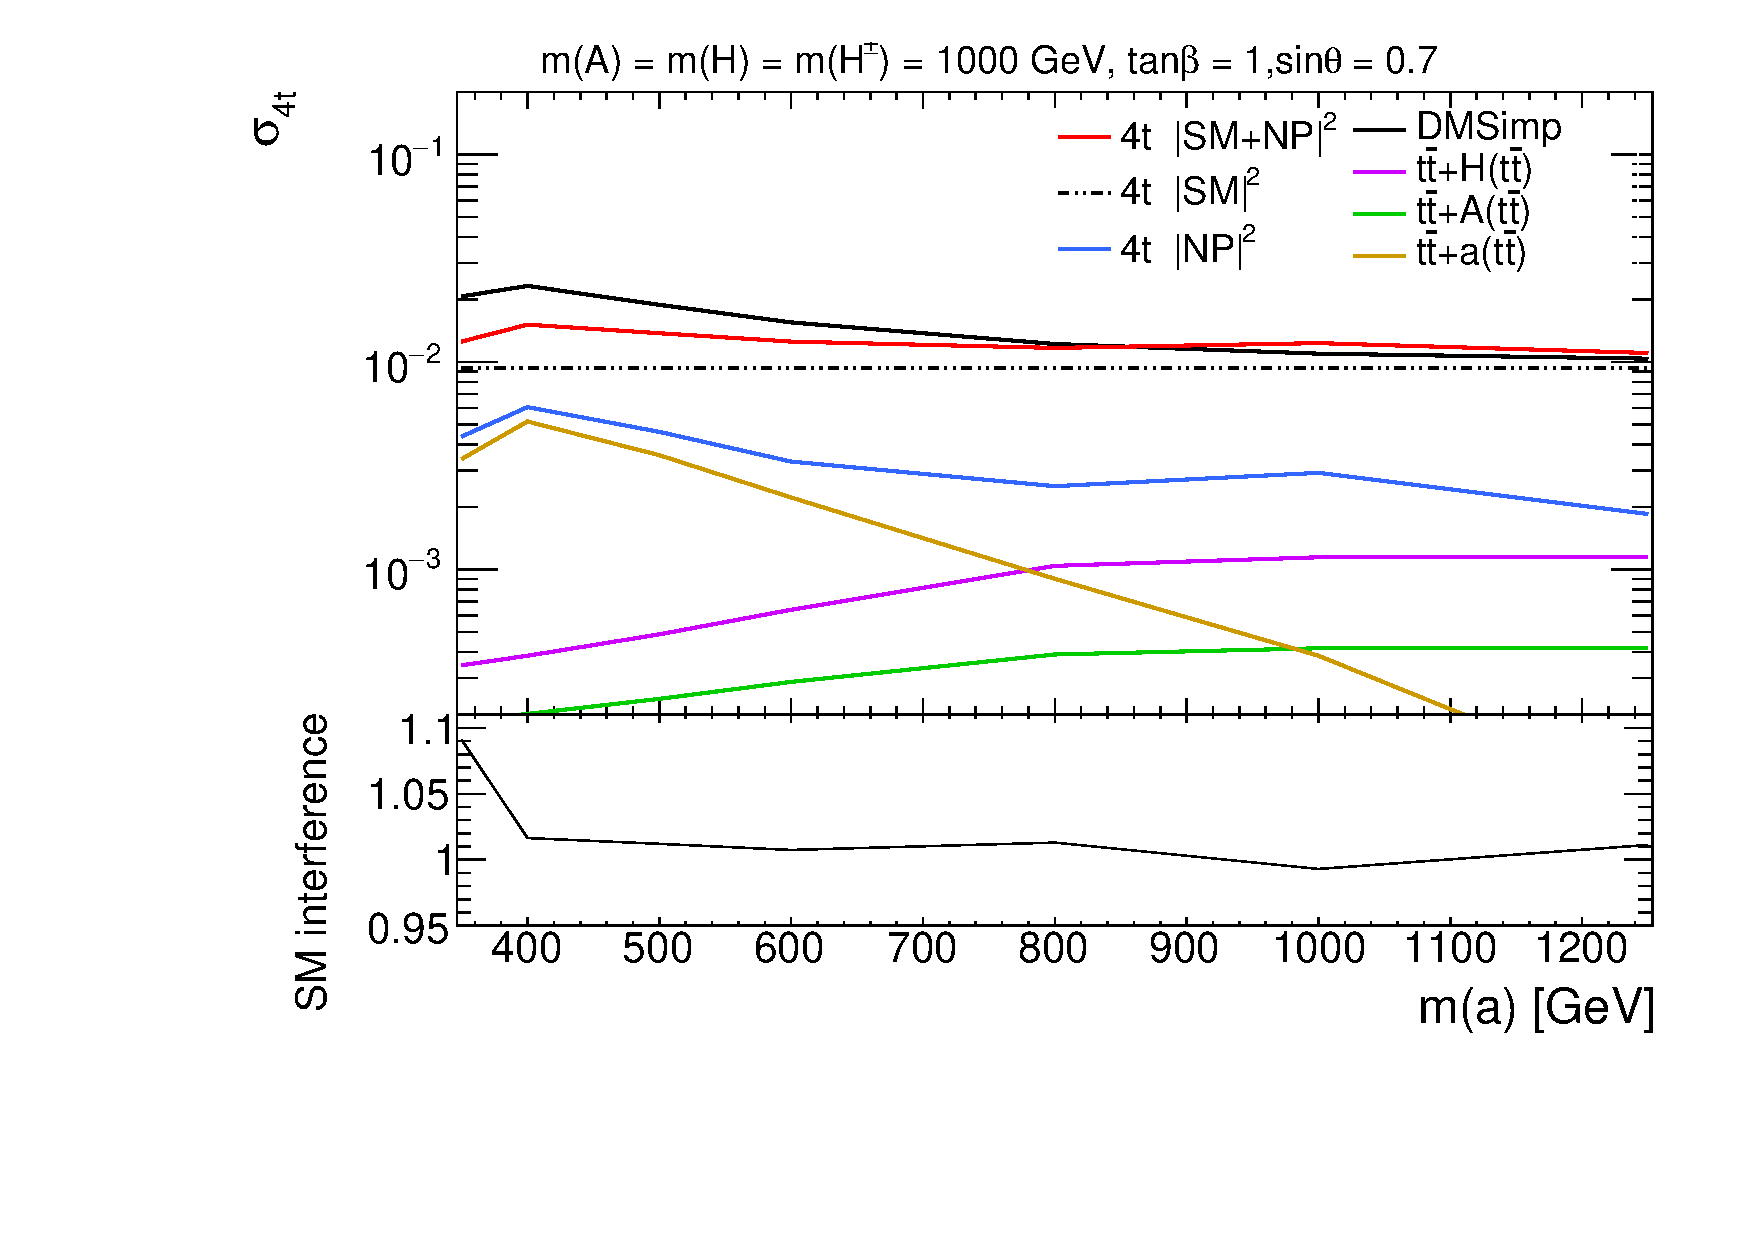
\includegraphics[width=\textwidth]{texinputs/04_grid/figures/DMHF/4tops/WHP_final_mascan.pdf}
\caption{}
\label{DMHF-4top-scan2}
\end{subfigure}
\caption{Four-top cross section study for a subset of the parameter space of benchmark \#2 (top) and \#3 (bottom). The different Standard Model (SM) and New Physics (NP) contributions with and without interference and the breakdown in terms of on-shell mediator
production is presented, following the notation of Table~\ref{tab-dmhf-4tops}. }
\end{figure}

\begin{figure}
\centering
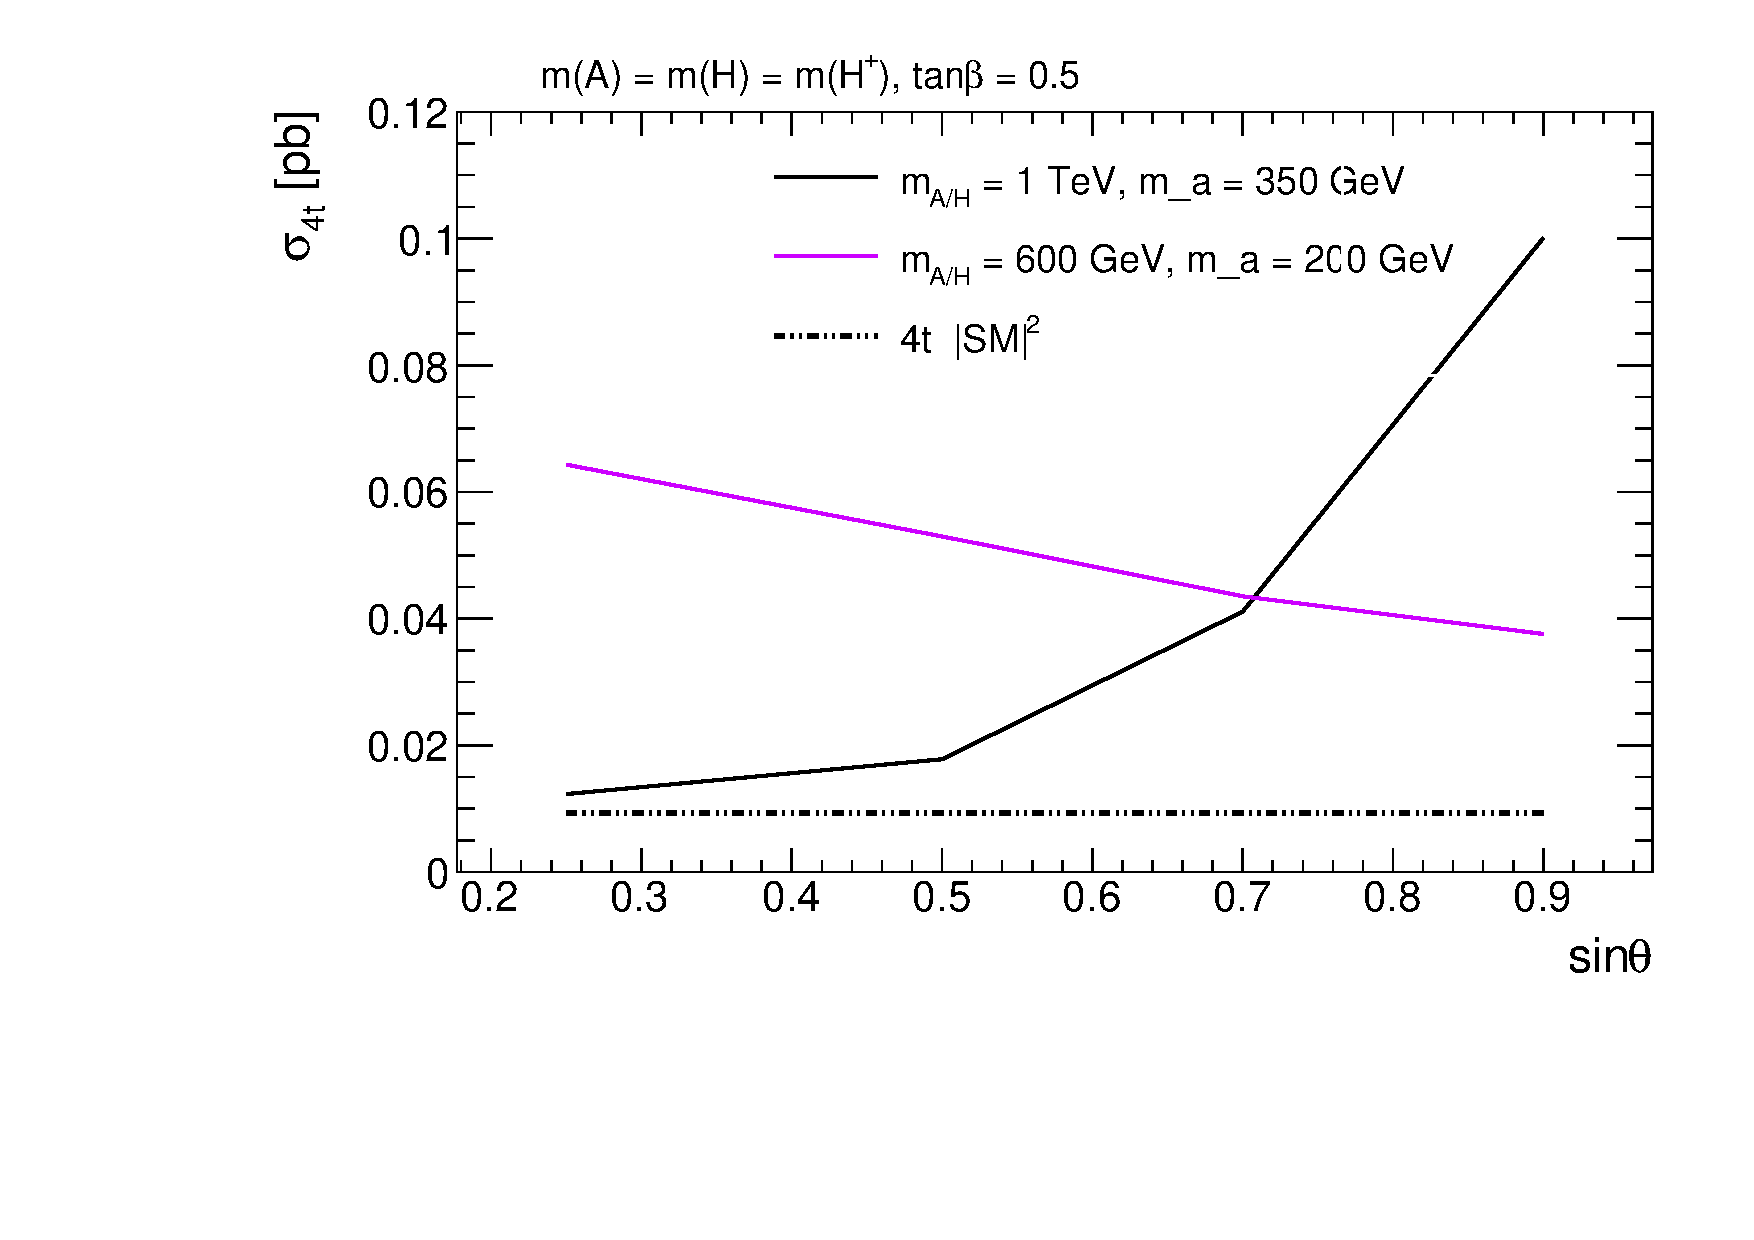
\includegraphics[width=.8\textwidth]{texinputs/04_grid/figures/DMHF/4tops/WHP_final_stscan.pdf}
\caption{Four-top cross section comparison for benchmarks \#3a and \#3b. Only NP contribution is presented, following the notation of Table~\ref{tab-dmhf-4tops}.}
\label{DMHF-4top-scan3}
\end{figure}

\FloatBarrier